\chapter{Exact Algorithm}
\label{sec:exact_algo}

\section{Overview}
\label{subsec:exact_algo_overview}

\begin{observation}
	\label{ob:frequency}
	A pair of subgraphs having higher support values can be expected to 
	have a higher correlation.
\end{observation}

\begin{observation}
	\label{ob:dfs}
	For highly (e.g., top-$k$) correlated subgraphs mining, generally a
	breadth-first or a best-first exploration of the search space is more
	efficient compared to a depth-first traversal of the search space.
\end{observation}

Setting $k$ to infinity would enable us to mine all pairs of correlated subgraph
patterns. However, on the contrary, it is hard to control the value of {\sf
Min-sup} to get the result of a particular $k$ of {\sf Top-$k$} correlated
subgraphs. That is to say, the {\sf Min-Sup} problem can be transfered from {\sf
Top-$k$} problem. As a result, we concentrate on {\sf Top-$k$} problem in the
following sections.

%% \setlength{\parskip}{0.3em}
% \spara{\raggedleft \textbf{Pattern Search Tree.}} 
\subsection{Search Tree}
\label{subsubsec:exact_algo_searchtree}
All operations including correlation computation and subgraph pattern extension
are performed on patterns following an exploration order on a \textit{search tree}.
We denote this tree by $T$. Each node $Q\in T$ represents a subgraph pattern. We
denote the set of current \textit{leaf} nodes in $T$ by $Leaf(T)$. At
every stage, a pattern $Q\in Leaf(T)$ that has not been \textit{operated} for correlation
computation is selected. Once operated, $Q$ is inserted into the
\textit{operated} set.

% Each element $Q_l\in Leaf(T)$ is a pattern that has not yet been $operated$ for correlation
% computation. A node $Q_l\in Leaf(T)$, once operated, is inserted into the
% $operated$ set.
% \setlength{\parskip}{0em}

% \subsection{Order of Subgraph Generation and Correlation Calculation}

\par The correlated subgraph mining algorithm is an iterative procedure,
essentially consisting of the following steps until convergence: 

\spara {\raggedleft \textnormal{1)}} Select a node $Q\in Leaf(T)$ that has not
been operated 

\spara {\raggedleft \textnormal{2)}} Calculate $\tau(Q,Q_j,h)$, \forall 
$Q_j\in \textit{operated}$ 

\spara {\raggedleft \textnormal{3)}} Extend $Q$ using possible single-edged
extensions to generate the set of "children" supergraphs of $Q$, \textit{children($Q$)}

\spara {\raggedleft \textnormal{4)}} Compute $\sigma(R),\ \forall R\in children(Q)$. If
$\sigma(R)\ge$ {\sf Min-Sup}, branch $T$ at $Q$ to include $R$ in $Leaf(T)$.

\begin{thrm}
	The order of subgraph generation and correlation calculation will not miss
	any correlated pairs between any of two frequent subgraphs.
\end{thrm}
% After step 4, we give $Q_i'$ an index of frequent subgraph discovery order,
% denoted as $index(Q_i')=a$, which means $Q_i'$ is the $a$-th subgraph in $T$.
% After the loop, we give $Q_i$ an index of correlation calculation order,
% denoted as $corIndex(Q_i)=b$, which means $Q_i$ is the $b$-th subgraph in $T$
% which and we put $Q_i$ into $Cor(T)$, i.e. $Cor(T)=Cor(T)\cap Q_i$.

\subsection{Best-first Search}
\label{subsubsec:exact_algo_bestfs}
Observation \ref{ob:frequency} suggests that faster convergence of the algorithm
could be expected if a subgraph pattern having a higher support is
\textit{operated} preceding every other unoperated pattern in $Leaf(T)$. As a result, we
use a heuristic to determine the priority of the leaf nodes in $Leaf(T)$
for processing: $Q_1$ has a higher priority than $Q_2$ \forall $Q_1, Q_2 \in Leaf(T)$ if and only if:
\begin{align*}\sigma(Q_1)>\sigma(Q_2)\end{align*}
Utilizing such a best-first heuristic, if leaf node $Q_k$ in the search tree has
the highest support among all other patterns in $Leaf(T)$, i.e. $\sigma(Q_k)=\max\{\sigma(Q_i)|Q_i\in Leaf(T),$ $Q_i$ $not$ $operated\}$, 
then $Q_k$ has the priorty to be operated and extended.
\par To implement best-first exploration, we introduce a priority queue called \textit{Search Queue} that simply queues,
 at any given time, all unoperated patterns in $Leaf(T)$ with the priority being accorded to patterns with higher frequencies. Also,
 note that as described in step $4$ of the algorithm outline in Section \ref{subsubsec:exact_algo_searchtree}, we do not consider 
 infrequent patterns in $Leaf(T)$, therefore, \textit{Search Queue} only orders frequent patterns. 

\subsection{Best-first Termination Criteria}
\label{subsubsec:exact_algo_ceasing}
Our objective is to mine $k$ pairs of correlated subgraphs and guarantee that any other pair of subgraphs cannot have a higher correlation $(\tau)$ than any pair in such a {\sf Top-$k$} list. 
A closer look at the properties mentioned in Section \ref{sec:characteristics} allows us to deduce the following: 
assume $Q$ and $Q_j$ are two arbitrary frequent subgraphs of the data graph. 
We denote $super(Q)$ as the set of all possible supergraphs of $Q$. Then, for all $Q'\in super(Q)$ the following conditions always hold:
\begin{align*} \tau(Q',Q_j,h)\le \sigma(Q') \quad $(\textsc{Corollary to Lemma \ref{lemma:prune}})$\end{align*}
\begin{align*} \sigma(Q')\le \sigma(Q) \quad \quad $(\textsc{downward-closure})$\end{align*}
It is easy to get the following upperbound on $\tau(Q',Q_j,h)$ by combining the two conditions above:
\begin{align*} \tau(Q',Q_j,h) \le \sigma(Q) \end{align*}
Consider this upperbound: if $\sigma(Q)$ is lower than the least $\tau$ value in
the {\sf Top-$k$} list, i.e. $\sigma(Q)<\tau(Q_a,Q_b,h)$ for all
pairs $Q_a,\ Q_b$ among the {\sf Top-$k$}, then all correlations
containing $Q\ (i.e.\ \tau(Q,Q_k,h))$ cannot
possibly be values in the {\sf Top-$k$} list. Furthermore, all correlation
values of every pattern $R$ with support values such that $\sigma(R)\leq
\sigma(Q)$ would also be ineligible for the list. Thus, in a best-first exploration
scheme, occurrence of such a case would signal termination of the search.


\par Another possible termination scenario exists wherein $k$ correlated pairs
do not even exist in the data graph. In this case, the size of the {\sf Top-$k$} list would be less than $k$ but there wouldn't exist
any frequent subgraph left in \textit{Search Queue} to operate.

\par Formally, we specify the two ceasing conditions for terminating search
based on a best-first heuristic:
\begin{align*} (1)\ \sigma(Q)\le min\{\tau(Q_a, Q_b, h)\ |\ (Q_a, Q_b)\in top\_k\},\ |top\_k|=k\end{align*}
\begin{align*}(2)\ Search\ Queue = \emptyset\end{align*}

In both these cases, we cease search and report all pairs of correlated
subgraphs discovered along with $\tau$ values. 

%\eat{
\begin{figure}[t!]
	\centering
	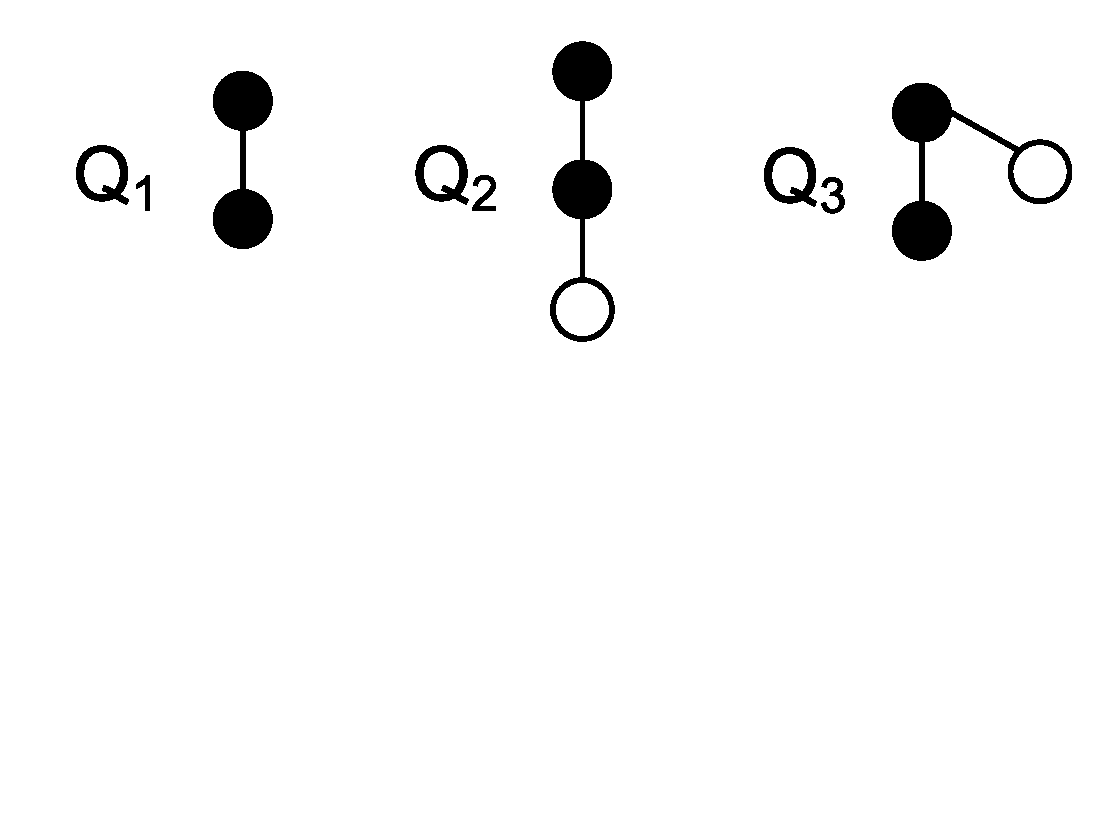
\includegraphics[scale=0.32]{images/ceasing_condition}
	\vspace{-2mm}
	\caption{\scriptsize For subgraphs $Q_1,Q_2,Q_3$, with $\sigma(Q_1)=5$,
	$\sigma(Q_2)=2$, $\sigma(Q_3)=3$. The current {\sf Top-$k$} $\tau$ values
	are $\{4,5,6\}$ for $k=3$, {\sf Min-sup}$=3$}.
	\label{fig:ceasing_condition}
	\vspace{-6mm}
\end{figure}
%}
\begin{exple}
	In Figure \ref{fig:ceasing_condition}, initially $Q_1$ is the
	only node in \emph{Search\ Queue} and $\sigma(Q_1)>4$. Suppose after
	$\tau$ calculations for $Q_1$, the minimum
	$\tau$ value among the {\sf top-$3$} pairs is $\tau{_{min}}=4$. After this,
	$Q_1$ is extended to $Q_2$ and $Q_3$. After extension, assume $\sigma(Q_2)<${\sf
	Min-sup} and $\sigma(Q_3)=$ {\sf Min-sup}. Thus, \emph{Search\ Queue} now only
	consists of $Q_3$ since $Q_2$ is not frequent. 
	But since $\sigma(Q_3)<\tau{_{min}}$ and there are already $3$ pairs in {\sf top-$k$}, i.e.
	$|top\_k|=3$ any correlation of $Q_3$ or $Q_2$ would not displace existing
	{\sf top-$k$} pairs. Thus, we cease search.
\end{exple}



\section{Replica-based Graph Instance Storage}
\label{subsec:replica-storage}
As discussed in Section \ref{sec:problem}, computing $\sigma$ and $\tau$
values requires knowledge of a pattern's \emph
{instances} (or \emph{isomorphisms}) in the
data graph. In a dense graph, the number of instances of a pattern can be
prohibitively large to store for each pattern so methods like \textsc{GrowStore} have limited
scope. In this section, we describe an elegant approach for performing subgraph
isomorphism using the \textbf{Replica Structure}.
 
\subsection{Replica Structure}
\label{subsubsec:replica-ds}
 Considering the large amount of overlaps of instances in dense graphs,
 we use a novel yet simple data structure to "store" all instances of a subgraph
 pattern, which not only solves potential memory issues that arise while
 tackling dense graphs, but also lays a robust foundation for carrying out
 efficient correlation calculations based on instance grouping (Section \ref{sec:problem}).
\par Instead of storing every instance of a pattern, we just create a reproduce
 of all occurrences of the vertices and the edges of the pattern in the data graph. We call the
 structure a \textit{replica} graph. We record all the vertex identifications
 and the edge connections in the \textit{replica} graph. In other words, a \textit{replica} graph is essentially a
 "minimal" subgraph \textit{G'} of data graph \textit{G} such that every
 instance of a pattern $Q$ in $G$ and every such instance only can be found in
 $G'$.
 
\eat{
\begin{figure}%[h!]
	% \vspace{-2mm}
	% \centering
	\begin{subfigure}[b]{0.25\textwidth}
		% \subfigure[{\scriptsize Subgraph Pattern $Q$}] {
		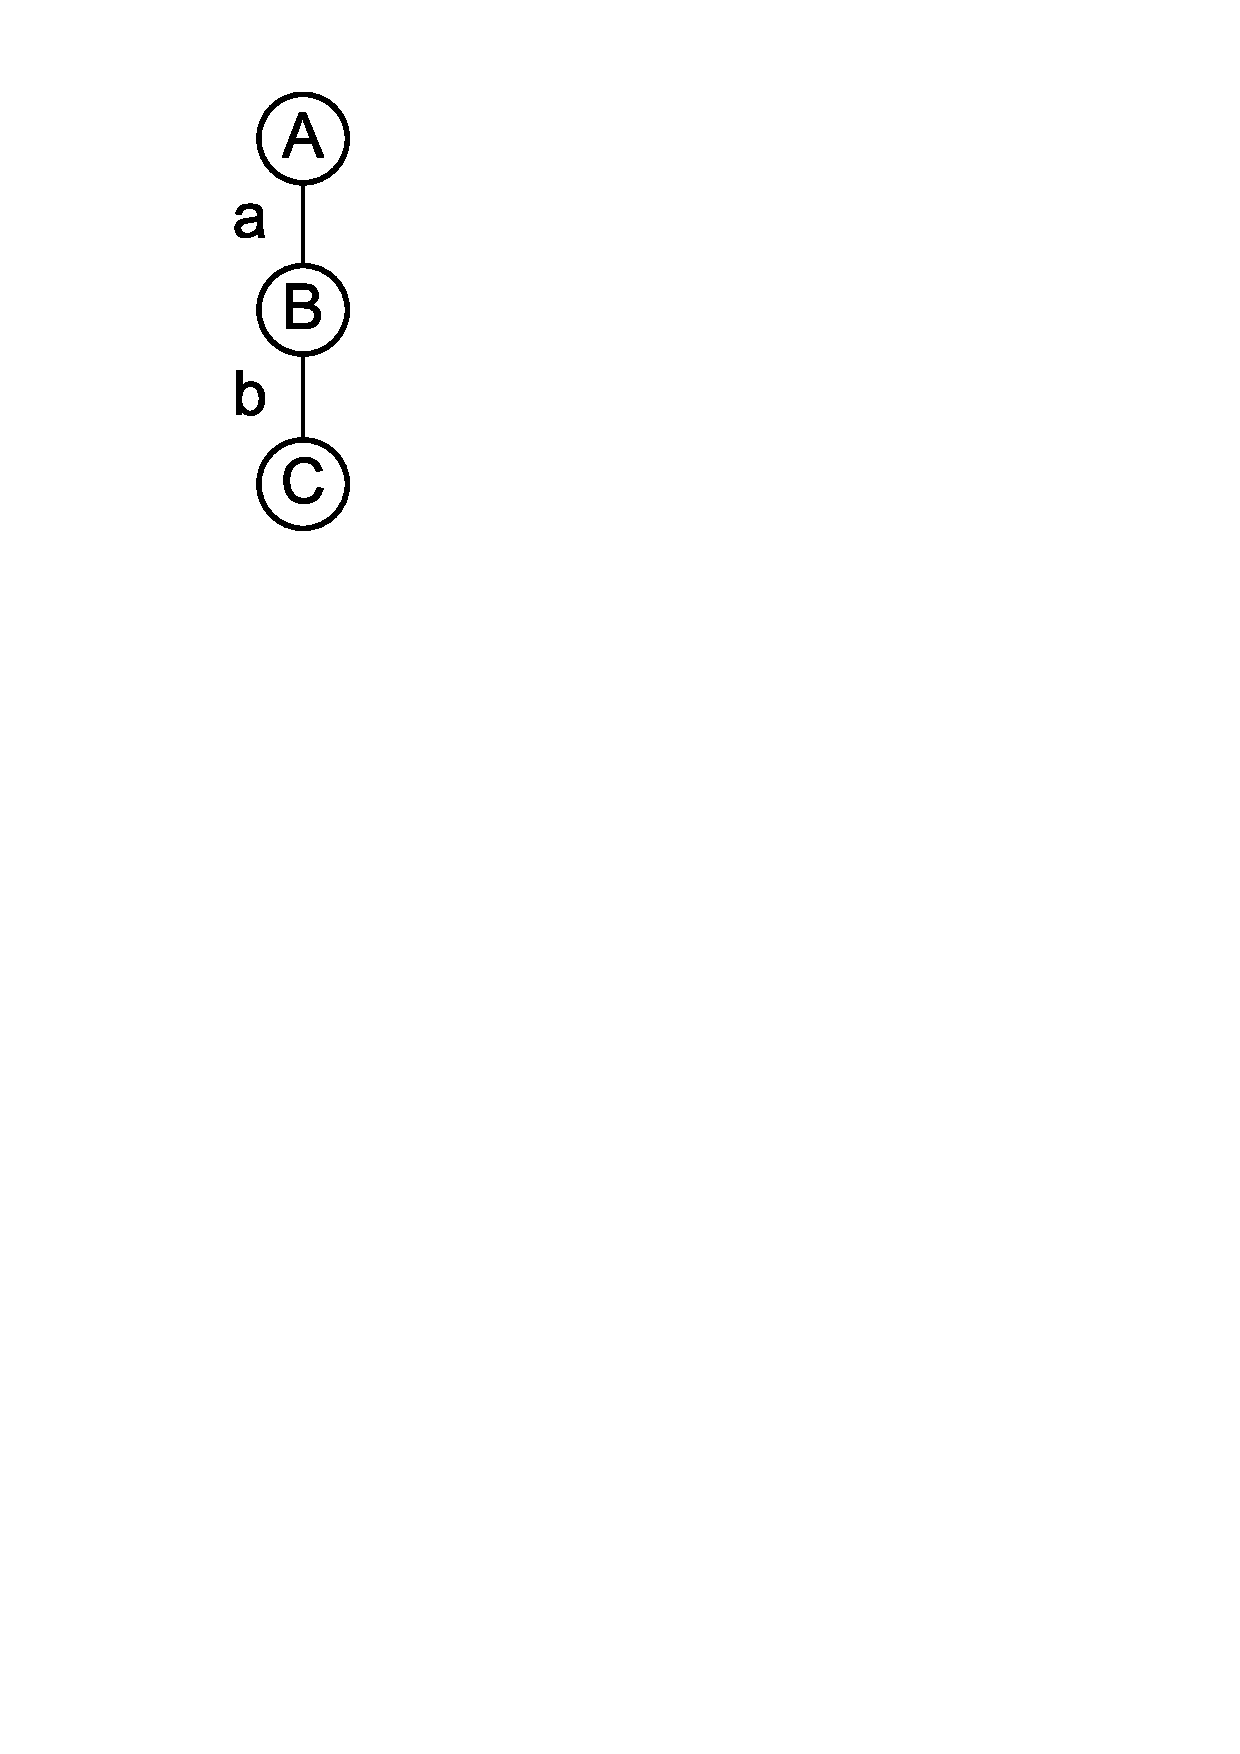
\includegraphics[scale=0.33]{images/replica1}
		\caption{}
		\label{fig:replica1}
		% }	
	\end{subfigure}
	% \begin{subfigure}
	% 	% \subfigure[{\scriptsize Occurrence of $Q$}]  {
	% 		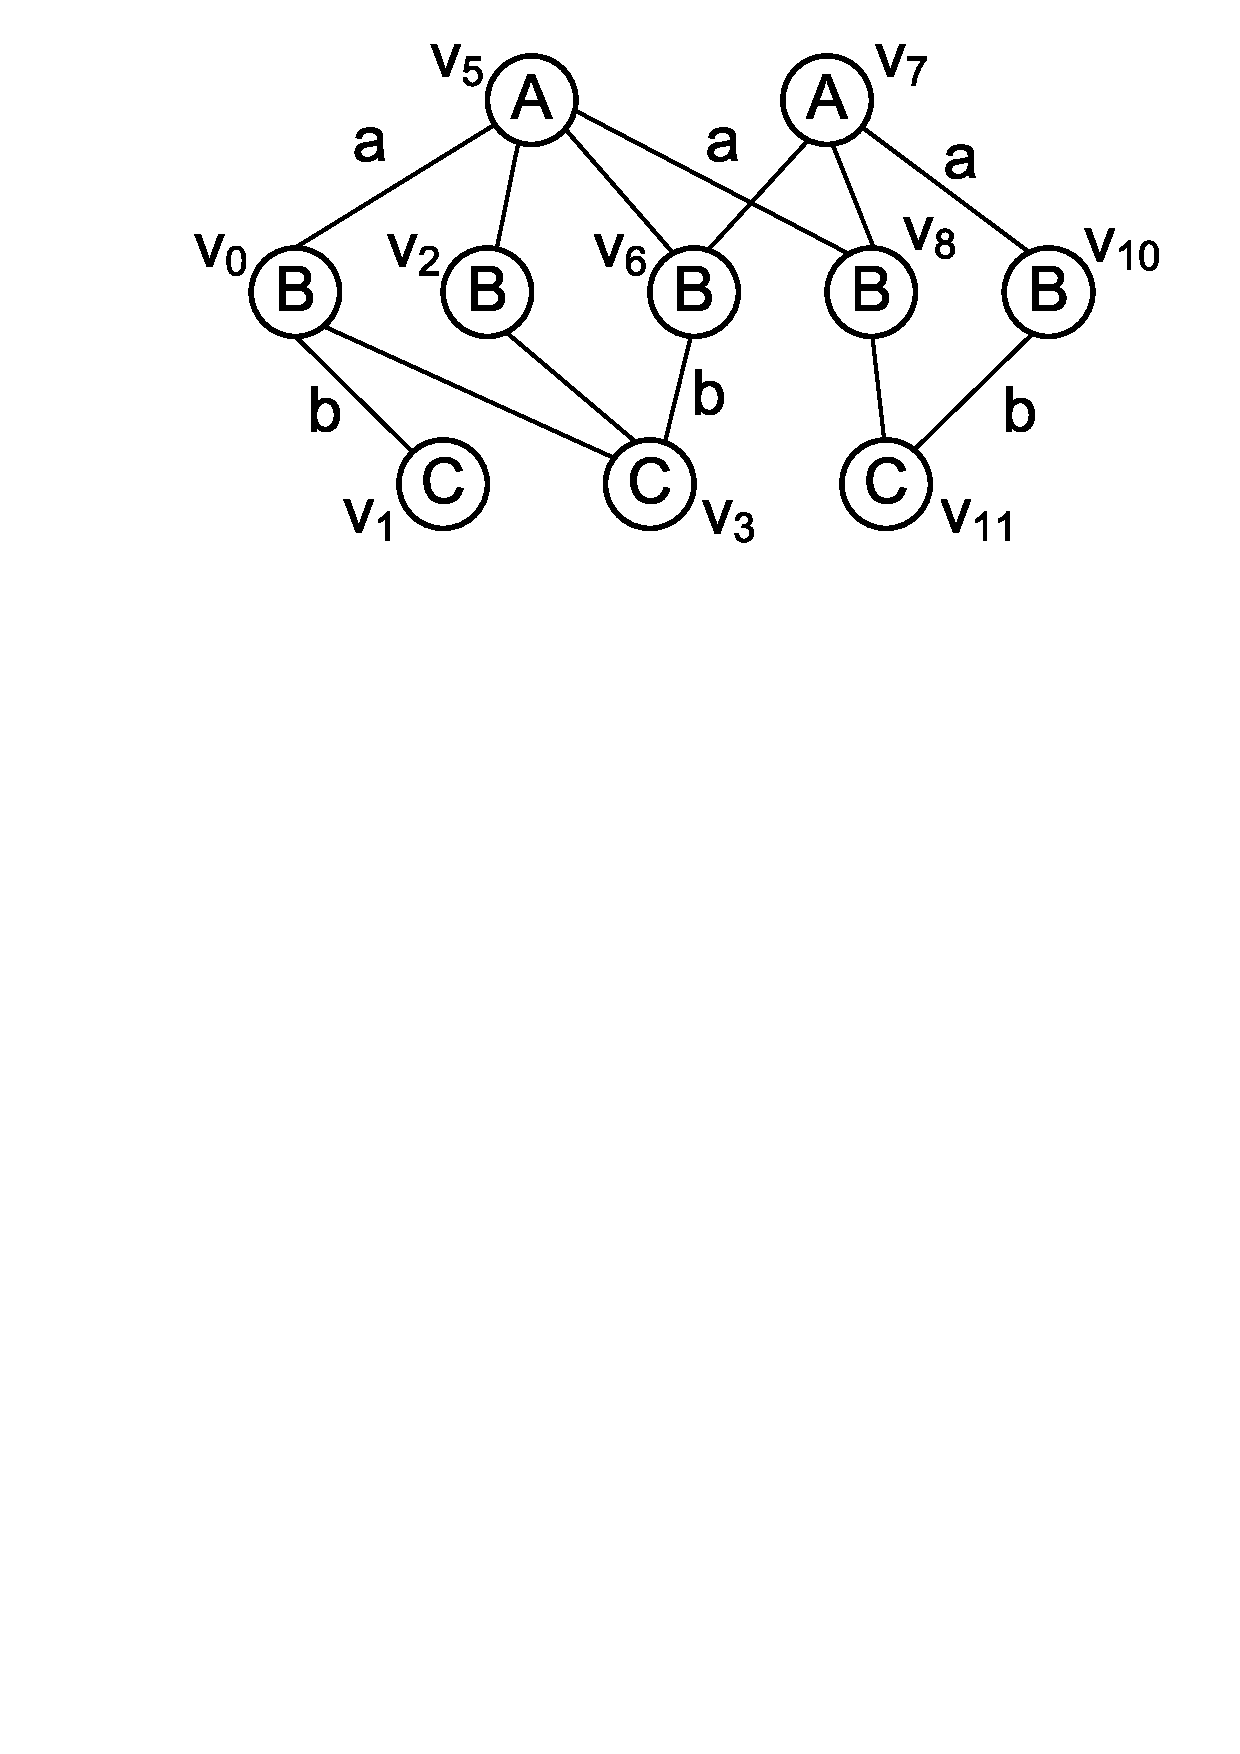
\includegraphics[scale=0.30]{images/replica2}
	% 		\label{fig:replica2}
	% 		\caption{}
	% 	% }
	% \end{subfigure}
	% \begin{subfigure}
	% % \subfigure[{\scriptsize Replica of $Q$}]  {
	% 	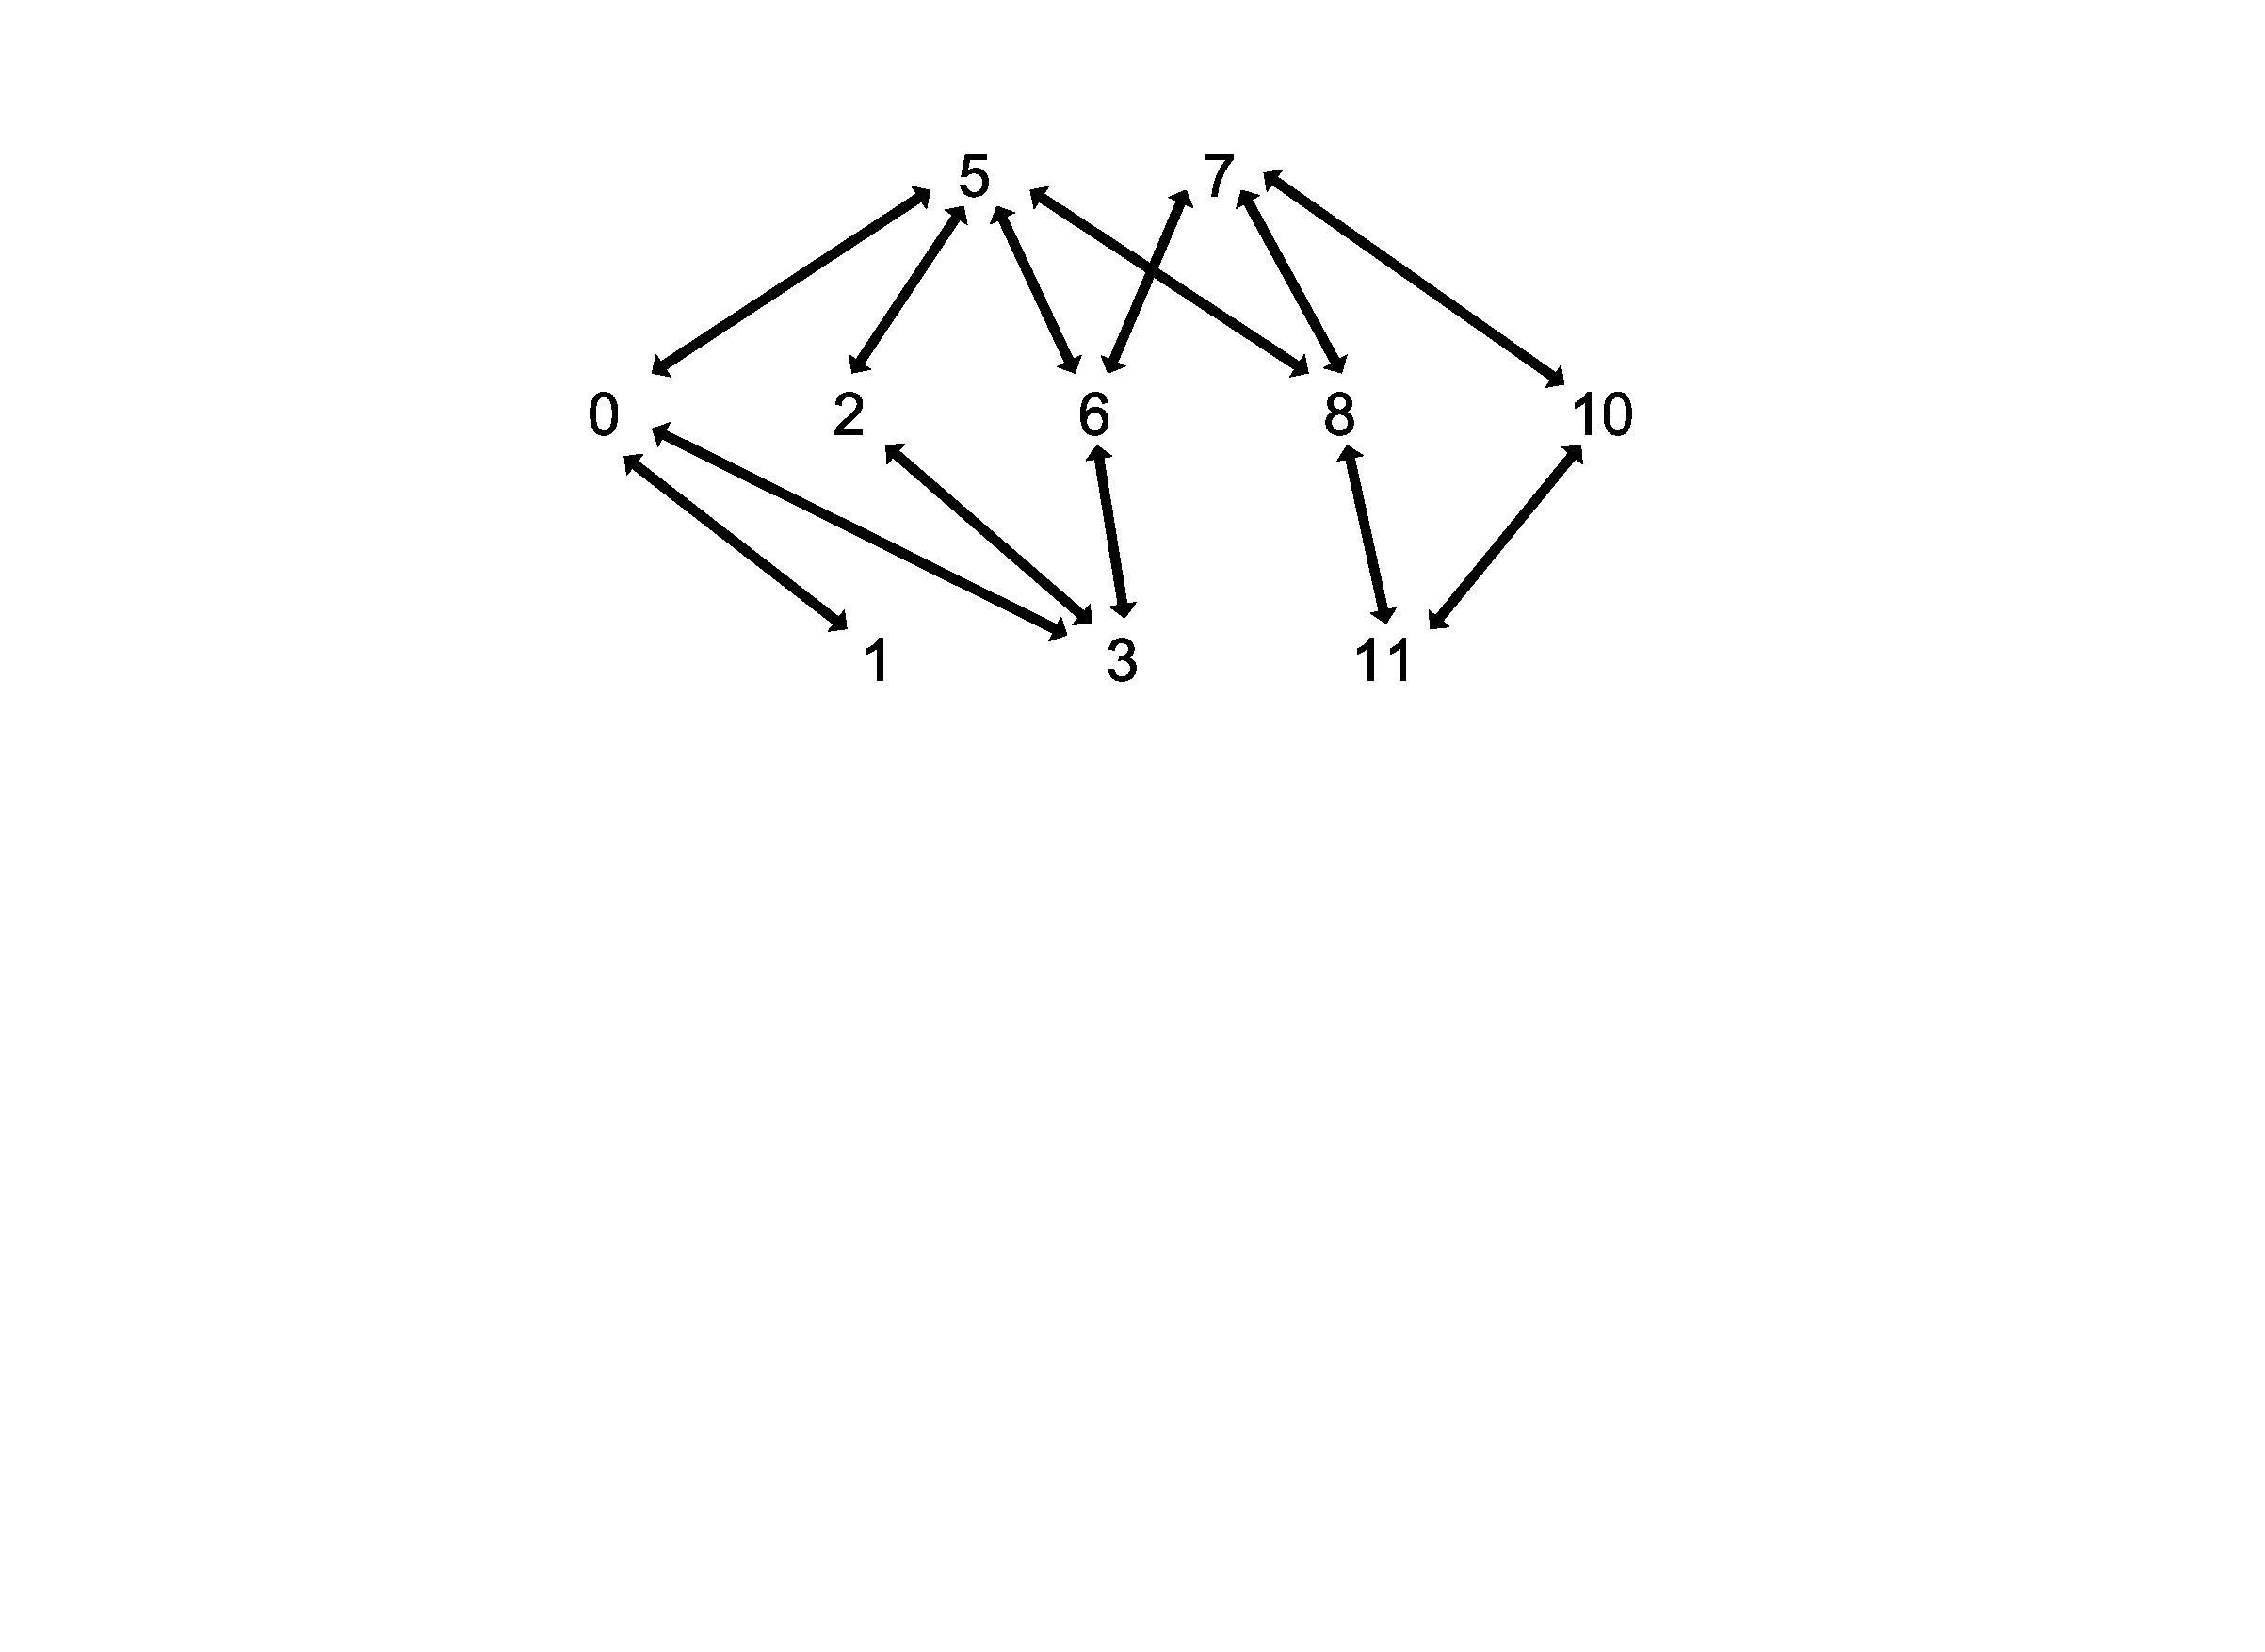
\includegraphics[scale=0.25]{images/replica3}
	% 	\label{fig:replica3}
	% % }
	% \end{subfigure}
	\vspace{-2mm}
	% \caption{\textsc{All the edge in Figure reffig:replica2 from $A$ to $B$, $B$ to $C$ has the edge label $a,b$ respectively. Figure reffig:replica3 is replicated from Figure reffig:replica2 without edge labels.}}
	\label{fig:replica}
	\vspace{-6mm}
\end{figure}
}
% \newline
\newline
% As {\sf Found($Q$)} occurs, we store the replica of $Q$ as a unit of the search tree. 

Figures \ref{fig:exactq} and \ref{fig:exactrepq} illustrate a pattern and its
corresponding \emph{replica} graph. A \emph{replica structure} consists of not
just the \emph{replica graph}, but also two maps, as
defined below. 

\eat{
After $Q$ has been $operated$, we remove $replica(Q)$ from memory.
}

\spara{\raggedleft Replica Structure.} Consists of the following three
structures constructed for each pattern $Q\in T$ for a data graph $G$:

\spara {\raggedleft \textnormal{1)}} \textit{Replica Graph}: occurrence
graph denoted by \textit{replica(Q)}

\spara {\raggedleft \textnormal{2)}} \textit{Mappings}: $\forall u \in
V(Q),\ Mappings(u, replica(Q))$ stores the set of all vertex identifications
$v\in V(replica(Q))$ of $u$

\spara {\raggedleft \textnormal{3)}} \textit{Inverse Mappings}: $\forall v \in
V(replica(Q)),\ InverseMappings$ $(v, Q)$ stores the set of all $u\in V(Q)$ such
that $v\in Mappings(u,$ $replica(Q))$

\spara {\raggedleft \textnormal{Both}} \emph{Mappings} and \emph{Inverse
Mappings} can be deduced from the \emph{replica} graph, however we still maintain
these indexes for computational gains. 


% \\2) For each $u_i\in Q$, there is a hash-map, $R_i(Q)$, recording the vertex
% identifications, and $R(Q)=(R_1(Q), R_2(Q), ..., R_{|V_Q|}(Q))$.
% \\3) For each element $v\in R_i(Q)$, there is a record of all the other vertices which $v$ is connected to in the occurrences of $Q$.

\subsection{Generation of a Replica Graph}
\label{subsubsec:replica-gen}
Algorithms 1 and 2 together describe the complete procedure to construct the
\emph{replica} structure for a subgraph pattern, henceforth referred to as
simply \emph{replica}. \emph{Replica} construction for any pattern $R$ requires
knowledge of the \emph{replica} of the pattern $Q$ that is extended to generate
it. Henceforth, we refer to such a pattern $R$ as a \textit{child} pattern of
$Q$ and $Q$ as the \textit{parent} pattern of $R$. Since the search procedure
processes a pattern only after its parent, the \emph{replica} of the
parent pattern can be used for constructing the \emph{replica} of the
child.
% \begin{algorithm}
% 	\DontPrintSemicolon
% 	\dontprintsemicolon
% 	\KwIn{Training sentences $S_{i}$}
% 	\KwOut{Sentence instances with cost-vectors for training $S_{i,c_i}$}
% 	\SetKwBlock{Begin}{function}{end function}
% 	\Begin($\text{generateCosts} {(} EV_{i,v,r} {)}$)
% 		{
% 	$S_{i,c_{i}} = \left[ \right]$\;
% 		\ForAll{$s \in S, v \in EV $}
% 		{
% 			$c_{i} = \left\lbrace \right\rbrace$\;
% 			set $region \; r = EV_{i,r}$\;
% 			\For{$p \leftarrow 1, properties$}
% 			{
% 				$c_{i,p} \coloneqq cost \left( kb_{r,p},v_{i,r} \right)$\;
% 				\uIf{$c_{p} > Cost_t$}
% 				{
% 					$c_{p} \coloneqq \infty$
% 				}
% 				\Else
% 				{
% 					continue
% 				}
% 			}
% 			\uIf{$\min \left( c \right)  > APE_t$}
% 			{
% 				$c_{i,no\_property} \coloneqq 0$
% 			}
% 			\Else
% 			{
% 				$c_{i,no\_property} \coloneqq \infty$
% 			}
% 			$\text{push} \left( S_{i,c_{i}}, \left( s,c_{i} \right) \right)$
% 		}\label{endfor}
% 		\Return{$S_{i,c_{i}}$}
% 	}
% 	\caption{Cost-Vector Algorithm}\label{costalgorithm}
% \end{algorithm}

\begin{algorithm}
	% \begin{algorithmic}[1] 
	% \REQUIRE input graph: $G$, parent pattern: $Q$, replica of $Q$: $replica(Q)$, extending index: $u$, tuple of extension vertex label and extension edge label: $candidate\ edge$, child pattern: $R$
	% \ENSURE all mappings of child pattern $R$ in $G$ (that is, the replica of $R$: $replica(R)$ in $G$)
	\dontprintsemicolon
	% \KwIn{Graph $G$, parent: $Q$, $replica(Q)$, extending index: $u\in V(Q)$, extension: $candidate\ edge$, child: $R$}
	\nonl \textbf{Input:} Graph $G$, parent $Q$, $replica(Q)$, child $R$, extending vertex: $u\in V(Q)$, extension: $candidate\ edge (u,v) \in E(R)$\;
	% \KwOut{$replica(R)$}
	\nonl \textbf{Output:} $replica(R)$ \;
	% \SetKwBlock{Begin}{function}{end function}
	% \Begin($\text{generateCosts} {(} EV_{i,v,r} {)}$)
	% {		
	$DFS\ List\leftarrow$ get rooted \textsc{DFS} of $Q$ with $u$ as $root$ \;
	$instance \coloneq \emptyset$\;
	\ForEach{ $u' \in Mappings(u,\ replica(Q))$}
	{
		$instance\leftarrow \{(u,u')\}$ \;
		\ForEach{\textup{edge} $e(u',v')\in E(G)$ \textup{that maps to} $candidate\ edge (u,v)$}
		{
			$instance\leftarrow instance \cup \{(v,v')\}$\;
			$\mathbb{I}\leftarrow$ \textsc{FindAllInstances($R$, $instance$, $\mathbb{I}$, $DFS\ List$, ...)}\;
			\textsc{UpdateReplica($replica(R)$, $\mathbb{I}$, ...)}\;
			$instance\leftarrow instance \setminus \{(v,v')\}$\;
			% Append all edges in $\mathbb{I}$ to $replica(R)$ and update the mappings list for every vertex\;
		}
		$instance\leftarrow instance \setminus \{(u,u')\}$\;
	}
	\Return{$replica(R)$}
	% }
	\caption{\textsc{GetReplica}}\label{algo:getreplica}
	% \end{algorithmic}
\end{algorithm}

Algorithm 1 essentially describes a backtracking procedure to find every instance (also referred to as
\emph{isomorphism} or \emph{mapping}) of the child pattern in the data graph $G$
using the mappings of the parent pattern and thus obtain its \emph{replica}. The
algorithm begins with a depth-first search ({\sf DFS}) procedure (line 1)
executed on the parent $Q$, selecting the vertex $u$ from which the
\emph{candidate edge} is extended as the \emph{root}. We call this vertex the
\textit{extending vertex} in $Q$. The \emph{edges} encountered in the {\sf DFS}
starting at $u$ are recorded in an ordered list called the \emph{DFS List},
which helps guide the isomorphism procedure performed subsequently. The
algorithm iterates over all mappings of $u$ in \emph{replica($Q$)} (line 3) and
attempts to find all (if any) instances of child $R$ in $G$ one-by-one. More
specifically, for every vertex $m \in V(replica(Q))$ that maps to the
\emph{extending vertex} $u$, the algorithm iterates over its adjacent edges $e
\in E(G)$ that map to the \emph{candidate edge} (line 5) and invokes
\textsc{FindAllInstances} (Algorithm \ref{algo:complete-instances}) to find
every instance of $R$ from \emph{replica($Q$)} that contains $e$. Algorithm
\ref{algo:complete-instances}, thus invoked, recursively enumerates all
instances of $R$ in a depth-first manner following the \emph{DFS List} of $Q$
(computed earlier). In the general case (lines 4-10), the algorithm begins by
invoking \textsc{NextQueryEdge} (line 4) which returns one edge at a time from
$E(Q)$ in the order of \emph{DFS List}. Edge $e(p,c)$ thus returned connects
vertices $p,c \in V(Q)$ such that $c\in children(p)$ in $Q$ as per the \emph{DFS
List} and $c$ is the pattern vertex to be matched next ($p$ is matched to $v \in
V(replica(Q))$). The algorithm then calls \textsc{FilterCandidates} (line 5) to
compute the the potential children set $P_c$ for storing all candidate vertices
$w\in V(replica(Q))$ for matching $c$ such that: (1) $w$ is contained in the
\textit{replica} graph adjacency list of $v$; (2) $c$ exists in the inverse
mappings set for $w$ in $replica(Q)$. That is, \forall $w \in P_{c}$, $c\in
InverseMappings(w)$; (3) The edge label of $(v,w)\in E(replica(Q))$ matches that
of $(p,c)\in E(Q)$. Next, for every vertex $w \in P_{c}$ such that $w$ has not
already been mapped to some other pattern vertex in the current
\textit{instance}, the algorithm attempts the mapping $(c,w)$ in
\textit{instance} (line 7) and recursively calls \textsc{FindAllInstances} (line
8) to match remaining pattern vertices following the \textit{DFS List} of edges.  

The \textit{Base Case} (lines 1-2) occurs when the algorithm finds an
\textit{instance} of $R$ (i.e., $|instance|=|V(R)|$) and returns it. The set of
all instances $\mathbb{I}$ thus found is returned at the end of Algorithm
\ref{algo:complete-instances} (line 10) and recorded by Algorithm
\ref{algo:getreplica} to update \textit{replica(R)} (lines 7-8, Algorithm
\ref{algo:getreplica}). In \textsc{UpdateReplica}, the algorithm simply appends
all edges and vertices of every instance in $\mathbb{I}$ to $E(replica(R))$ and
$V(replica(R))$ respectively and also updates the \textit{Mappings} and
\textit{InverseMappings} indexes for every vertex of pattern
$R$ to include the vertices of the newly-discovered instances in corresponding sets
and vice-versa.
% The {\sf find all instances()} function used in Algorithm ? is defined below.
% It enumerates all instances in a depth-first manner starting from the
% $extending\ index$ as the $root$ by following the {\sf DFS} edge-ordering
% stored in $DFS\ List$.
\begin{algorithm}
	\dontprintsemicolon
	\caption{\textsc{FindAllInstances} \textsc{(Exact)}}\label{algo:complete-instances}
	\nonl \textbf{Input:} Graph $G$, parent $Q$, $replica(Q)$, child $R$, $DFS$ $List$, partial isomorphism of $R$: $instance$, $\mathbb{I}$\;
	% parent edge: $(u, v)\in E(G)$ mapped to $(u',v')\in E(R)$,
	% \KwOut{$replica(R)$}
	\nonl \textbf{Output:} $\mathbb{I}: $ set of all instances of $R$ in $G$ consistent with input partial isomorphism $instance$\;
	%such that $\forall I \in \mathbb{I} $  $ (u',u),(v',v) \in I$)\;
	% \REQUIRE input graph: $G$, parent pattern: $Q$, replica of $Q$: $replica(Q)$, parent edge: $(u, v)$, $DFS\ List$ of $Q$ rooted at $extending\ index$, child pattern: $R$
	% \ENSURE all mappings of pattern $R$ in $G$ that include $(u, v)$
	\uIf{$|instance|=|V(R)|$}
	{
		\Return{$instance$}
	}
	\Else
	{
		$e(p,c) \coloneq$ \textsc{NextQueryEdge($DFS\ List, ...$)}\;
		$P_{c} \coloneq$ \textsc{FilterCandidates($instance, c, ...$)}\;
		\ForEach{$w \in P_{c}$ \textup{such that w is not yet matched}}
		{
			$instance \leftarrow instance \cup \{(c,w)\}$\;
			$\mathbb{I} \leftarrow \mathbb{I}\ \cup$ \textsc{FindAllInstances($R,instance,$ ...)}\;
			$instance \leftarrow instance \setminus \{(c,w)\}$\;
		}
		\Return{$\mathbb{I}$}\;
	}
	% \IF{all $edges$ in $DFS\ List$ have been mapped}
	% \STATE \textbf{return} $instance$ set
	% \ENDIF
	% \FORALL{adjacent edges $e$ of $v$ in $replica(Q)$}
	% \IF{$e$ maps to the corresponding $child\ edge$ in $DFS\ List$ \textbf{and} \textbf{not} already in $instance$}
	% \STATE $instance\leftarrow instance\cup e$
	% \STATE $\mathbb{I}\leftarrow \mathbb{I}\ \cup\ ${\sf find\ all\ instances($R$, $e$, $instance$, $DFS\ List$)}
	% \STATE $instance\leftarrow instance \setminus e$
	% \ENDIF
	% \ENDFOR
	% \STATE \textbf{return} $\mathbb{I}$
\end{algorithm}

This replica-based instance storage strategy not only builds a foundation for the sequential
efficient correlation calculation, but also benefits the MNI support counting in
the single large graph since we can directly get $\sigma(R)$ when we record the
\textit{replica(R)} just by counting all the sizes of the $Mappings(v)$, where $v\in
V(Q)$.

% \textcolor{red}{#to be added: !replica(R) can be deleted after operate(R)-memory benefit}

% \subsubsection{\textcolor{red}{?}Indexing to Facilitate Replica Deletion}
% \label{subsubsec:replica-indexing}


\begin{figure*}
    % \captionsetup[subfigure]{oneside, margin={0.4cm,0cm}}
    % \captionsetup[subfigure]{labelfont=normalfont,textfont=normalfont,singlelinecheck=on,justification=raggedright, skip=20pt}
    %, skip=-10pt}
	\begin{subfigure}[b]{0.15\textwidth}
            % \centering
            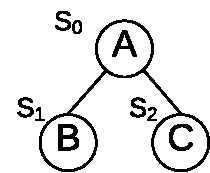
\includegraphics[scale=0.6]{img_ex/Exact-Q.pdf}
            \caption{}
			\label{fig:exactq}
    \end{subfigure}%
    % \hspace*{\fill}
    % \captionsetup[subfigure]{labelfont=bf,textfont=normalfont,singlelinecheck=on,justification=raggedright, skip=-5pt}
	\begin{subfigure}[b]{0.35\textwidth}
            % \centering
            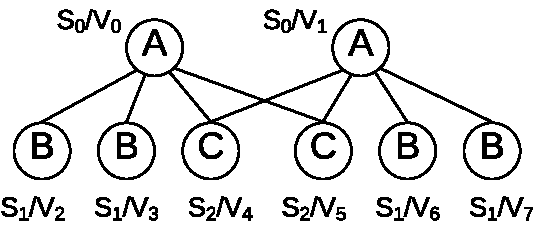
\includegraphics[scale=0.6]{img_ex/Exact-rep(Q).pdf}
            \vspace{-1.3\baselineskip}
            \caption{}
			\label{fig:exactrepq}
	\end{subfigure}
	\captionsetup[subfigure]{skip=-2pt}
	\begin{subfigure}[b]{0.15\textwidth}
		% \centering
		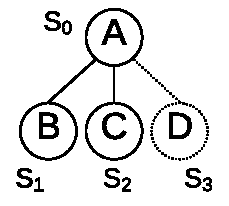
\includegraphics[scale=0.6]{img_ex/Exact-R.pdf}
		\caption{}
		\label{fig:exactr}
	\end{subfigure}%
	% \hspace*{\fill}
	\begin{subfigure}[b]{0.35\textwidth}
		% \centering
		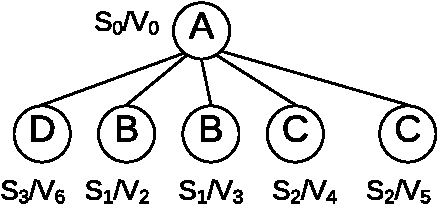
\includegraphics[scale=0.6]{img_ex/Exact-rep(R).pdf}
		% \vspace{-1.3\baselineskip} %not needed because figures are aligned
		% naturally unline above case
		\caption{}
		\label{fig:exactrepr}
	\end{subfigure}
	% \captionsetup[figure]{skip=200pt}
    \vspace{0.5\baselineskip}
	\caption{\textup{(a)} parent $Q$ \textup{(b)} $replica(Q)$ \textup{(c)} child $R$ showing edge extension $(S_0, S_3)$ \textup{(d)} $replica(R)$}\label{fig:exactex}
	\vspace{0.75\baselineskip}
\end{figure*}

\begin{exple}	
	In Figure \ref{fig:exactex}, originally \emph{Q} and \emph{replica(Q)} are
	as shown in \ref{fig:exactq} and \ref{fig:exactrepq} respectively. Child
	\emph{R}, extended from \emph{Q} at \emph{extending vertex} $S_0$ using the
	\emph{candidate edge} $(A, D)$ is as shown in \ref{fig:exactr}. Assume
	\emph{DFS List} starting at $S_0$ records edges $(S_0, S_1)$ and $(S_0,
	S_2)$ in that order. To construct \emph{replica(R)}, the algorithm jumps to
	$Mappings(S_0)$ in \emph{replica(Q)}, i.e. ${V_0}$ followed by ${V_1}$.
	Assume, $(V_0, V_6), (V_0, V_7)\in E(G)$ map to $(A, D)$ but no such
	mapping edges exist incident to $V_1$ in $G$. All instances of $R$ thus found
	would result in \emph{replica(R)} as shown in Fig.\ref{fig:exactrepr}
\end{exple}

\section{Subgraph Extension}
\label{subsec:subgraph-ext}
\subsection{Extension Rule}
We assign pattern vertex indices for all $V_i\in V(Q)$ to identify their order of discovery.
\begin{defn}[Vertices Subscripting] For all $Q\in T$, apart from vertex
	identification $V_i$, we use another convention to label the vertices in $Q$
	by the \textbf{order} of discovery leading to pattern $Q$, denoted as
	$S_Q=(S_0,S_1,...,S_n)$, $n=|V_Q|$. Thus, $\forall S_i, S_j$, if $i<j$, then
	the vertex $V_i$ is discovered earlier than the vertex $V_j$.
\end{defn}

Taking advantage of this convention, it is easy to get the right-most path of a
subgraph. $Q$ is then extended only from vertices along the right-most path in
single-edged extensions to generate $children(Q)$ which continue the search. Algorithm
\ref{algo:extension} captures this procedure.

\begin{algorithm}
	\dontprintsemicolon
	% \begin{algorithmic}[1]
	\nonl \textbf{Input:} Graph $G$, parent $Q$, $replica(Q)$ \;
	\nonl \textbf{Output:} $Ex(Q)$: set of candidate edge extensions for $Q$\;
	% \REQUIRE data graph $G$, subgraph pattern $Q$, replica of $Q$, {\sf Min-sup}
	% \ENSURE frequent pattern set extended from $Q$, $Ex(Q)$
	$Ex(Q)\coloneq \emptyset$ \;
	$rmpath \leftarrow$ right-most path of $Q$ from $DFS\ Code(Q)$\;
	\ForEach{$v\in rmpath$}
	{
		\ForEach{$v'\in Mappings(v,replica(Q))$}
		{
			$E\leftarrow$ set of all edges $(v',w')\in E(G)$ extending $Q$\;
			$Ex(Q)\leftarrow Ex(Q)\cup E$
		}
	}
	\Return{$Ex(Q)$} 
	% \STATE $Ex(Q)\leftarrow\emptyset$
		% \STATE $Rmpath\leftarrow$ right-most path of $Q$
		% \FORALL{$s$ in $Rmpath$}
		% \STATE $Ex(Q)\leftarrow Ex(Q)\cup$ possible extensions
		% \ENDFOR
		% \FORALL{$ex$ in $Ex(Q)$}
		% \IF{$\sigma(ex)<$ {\sf Min-sup}}
		% \STATE $Ex(Q)\leftarrow Ex(Q)\setminus ex$
		% \ENDIF
		% \ENDFOR
		% \RETURN $Ex(Q)$
	% \end{algorithmic}
	\caption{\textsc{SubgraphEdgeExtensions}}\label{algo:extension}
\end{algorithm}

\textsc{SubgraphEdgeExtensions} iterates over every mapping $v'\in
V(replica(Q))$ for every $v\in rmpath($Q$)$ and attempts to extend $Q$ using a
single-edge extension. The set of all valid candidate edge extensions, $Ex(Q)$ thus
obtained is returned. 

\subsection{Duplicated Subgraph Prunning}
To avoid the duplicated subgraph judgement, we take the advantage of the DFS
code, and the minimum DFS code in gSpan\cite{YH02}, whenever a subgraph is
constructed we compute its minimum DFS code, denoted as $DFS\ Code(Q)$.

\par We use a dictionary $\mathbb{D}$ to store all the minimum $DFS\ codes$ we have
discover. When a subgraph $Q$ is discovered, we perform a lookup for $DFS\ Code(Q)$ in the
dictionary. If $DFS$ $Code(Q)$ $\in$ $\mathbb{D}$, then $Q$ must have been discovered before,
so we prune $Q$.

% \textcolor{red}{completeness theorem pending}

\section{Correlation Computation}
\label{subsec:corrcomp}

\subsection{Global Index}
\label{subsec:global-index}

We use a global index to record all the distance information. Each vertex of the data graph stores two catogories of distance information.

\squishlist
\item{\bf Proximity Vertices.} For each $u\in G$, we store the information of proximity vertices of $u$, denoted as $CorV(u)$, for each vertex $u\in CorV(u)$, there exists $d(u,v)\le h$.
\squishend
\squishlist
\item{\bf Proximity Patterns.} For each $u\in G$, we store the information of proximity patterns of $u$, denoted as $CorP(u)$, for each pattern $Q\in CorP(u)$, suppose the instance-groups of $Q$ is $\mathbb{I'}=\{I'_1,I'_2,\ldots,I'_{\sigma(Q)}\}$, there exists $I'\in \mathbb{I'}$, $\exists v\in I'$, $d(u,v)\le h$.
\squishend
With the global index acquired before the search, there is no need to consider anything about the distance (hop-constraints) in the search steps. The detail of the maintenance of these two indices is specified in Section \ref{subsec:calculating}.

\subsection{Calculating Correlation}\label{subsec:calculating}
\begin{defn}[Positive Instance Group]
	Given two subgraphs $Q_1$ and $Q_2$ in the input graph $G$, their instance-groups
	$\mathbb{I'}=\{I'_1,I'_2,\ldots,I'_{\sigma(Q_1)}\}$ and $\mathbb{J'}=\{J'_1,J'_2,\ldots,J'_{\sigma(Q_2)}\}$,
	respectively, and a user-defined distance-threshold $h$, assume that $\sigma(Q_1) \le \sigma(Q_2)$.
	Then, we say an instance group of $Q_1$, $I'_i\in \mathbb{I'}$ is a {\bf positive instance group} of $Q_2$ if following condition is satisfied.
	%
	\begin{align}
		\exists J' \in \mathbb{J}, \exists u \in I', \exists v \in J', d(u,v)\le h
	\end{align}
	Then, we denote $P(I'_i,Q_2,h)=1$, otherwise $P(I'_i,Q_2,h)=0$.
\end{defn}
\begin{thrm}
	Let $Q_1,Q_2$ be two subgrpah patterns, and an instance group of $Q_1$, $I'$. Then,	if $Q_2\in \cap CorP(v),v\in I'$, $P(I'_i,Q_2,h)=1$.
	otherwise, $P(I'_i,Q_2,h)=0$.
\end{thrm}
The process of correlation calculation could be considered as a {\bf collection}. Suppose we are calculating the correlation of $Q_1$, i.e. $\tau(Q_1,Q_k,h)$, for all $Q_k\in Cor(T)$. Taking advantage of the global index in Section \ref{subsec:global-index}, by traversing all the vertices in a group can we know the correlation $\tau()$ of all the $v$. We collect these sets one-by-one and finally we could know all the correlation of $Q_1$, i.e. $\tau(Q_1,Q_k,h)$, for all $Q_k\in Cor(T)$.

\subsection{Replica Structure Transformation}
It is more convenient to implement an efficient collection in a hierarchical structure, like tree. As a result, to initialize a collection, we first transform the search space of the collection to a particular tree.
\par Prior to the detailed operations, we first define the group center and the collection tree of a pattern.
\begin{defn}[Group Center and Center Subscript]
	Given a subgraph $Q$, and the instance-groups of $Q$, $\mathbb{I'}=\{I'_1,I'_2,\ldots,I'_{\sigma(Q)}\}$, a group center $u$ of $I'_i$ is the vertex having the minimum MNI support among all $v\in I'_i$, denoted as $u=center(I_i)$, a center subscript is the vertex subscript has the MNI support of the images, denoted as $centerSubscript(Q)$. i.e. $centerSubscript(Q)=i$, where $M(s_i)=\sigma(Q)$.
\end{defn}
\begin{defn}[Collection Tree]
	Given a subgraph $Q$, a collection tree of $Q$, $CT(Q)$ is tree transfromed from the tree structure replica, and rooted at $centerSubscript(Q)$.
\end{defn}
% First of all, if a subgraph contains any backward edges, we remove all its backward edges in its replica prior to the calculation. This is because 1) removing backward edges would not affect the result of correlation calculation. 2) removing backward edges could derive a tree structure subgraph, which is more convenient to carry out the collection.
% \eat{
\begin{figure}[t!]
	\vspace{-2mm}
	\centering
	\eat
	{
		\subfigure[{\scriptsize Subgraph Pattern $Q_1$}] {
			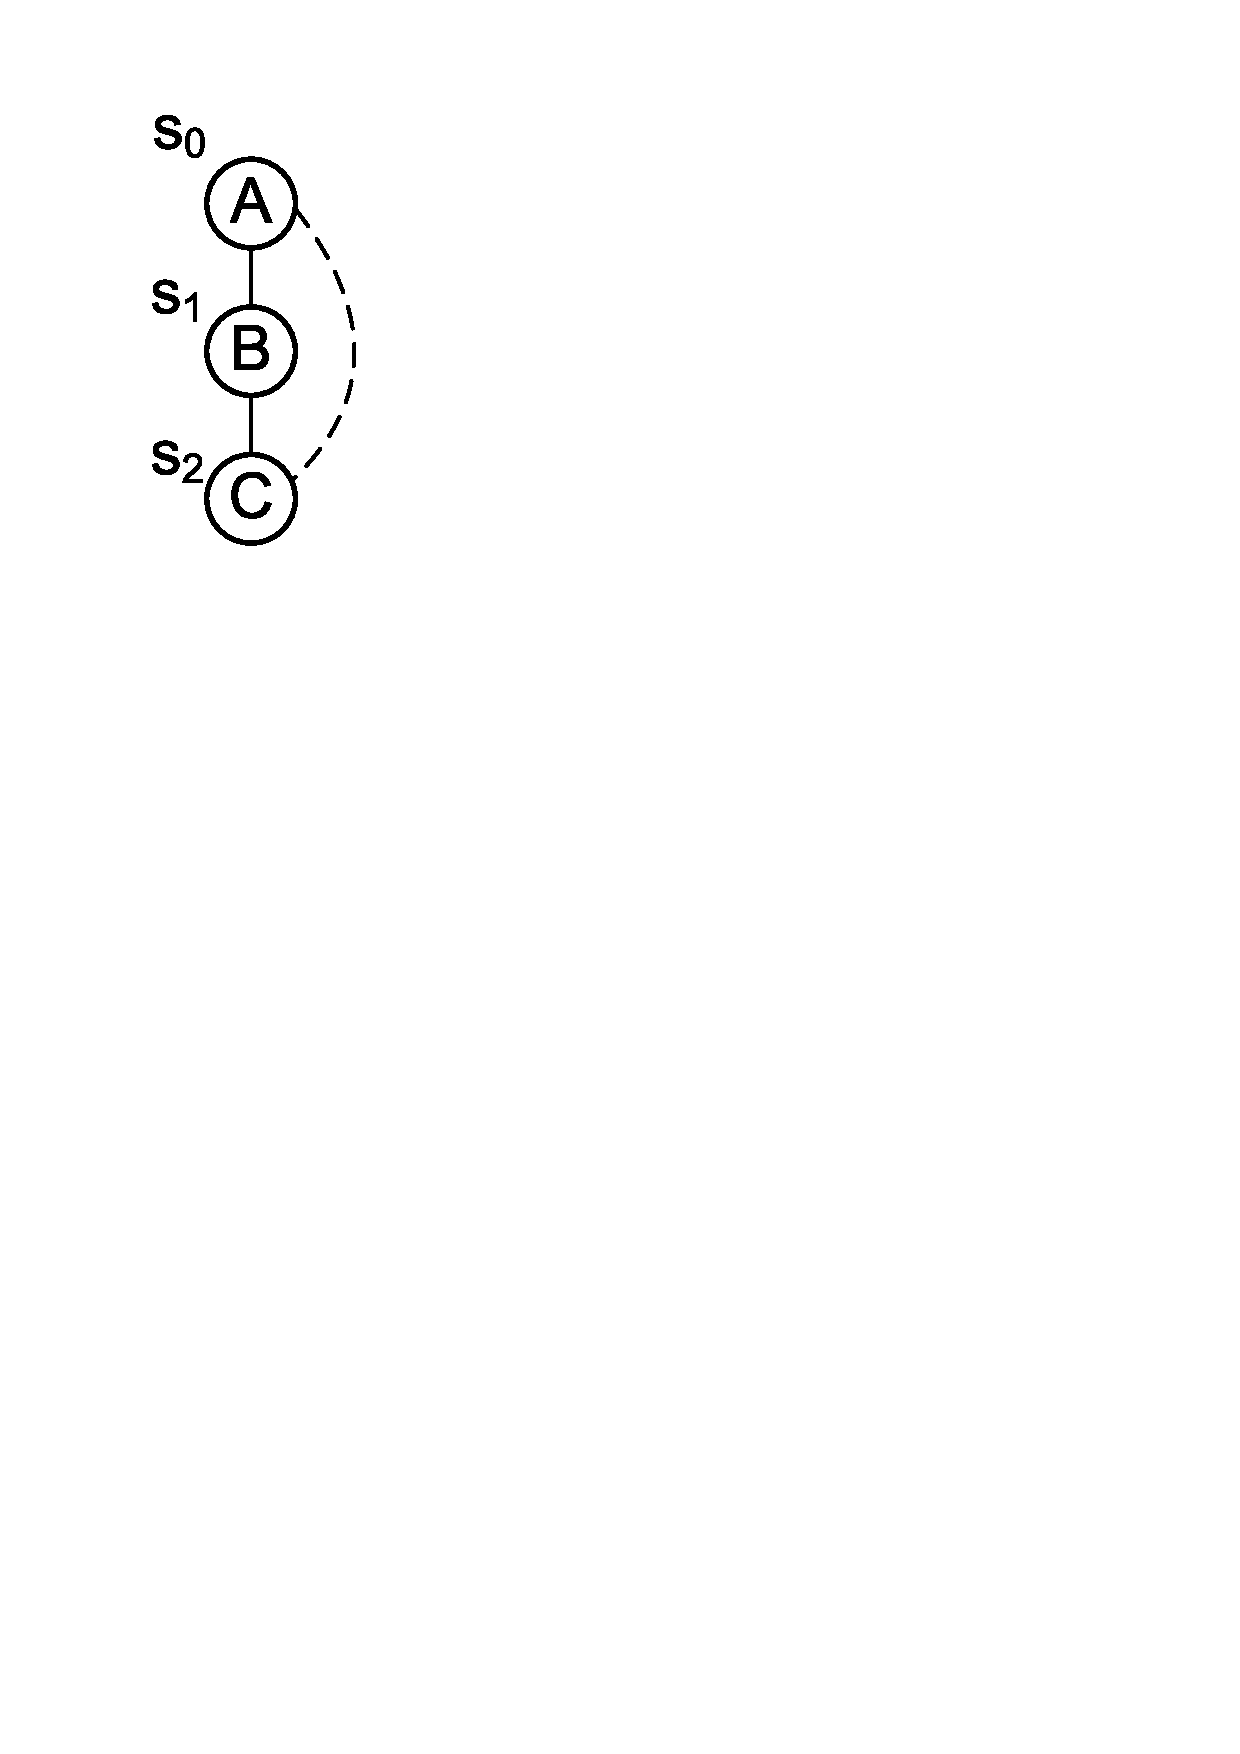
\includegraphics[scale=0.35]{images/tree_structure0}
			\label{fig:tree_structure0}
		}
		\subfigure[{\scriptsize Occurrence of $Q_1$}] {
			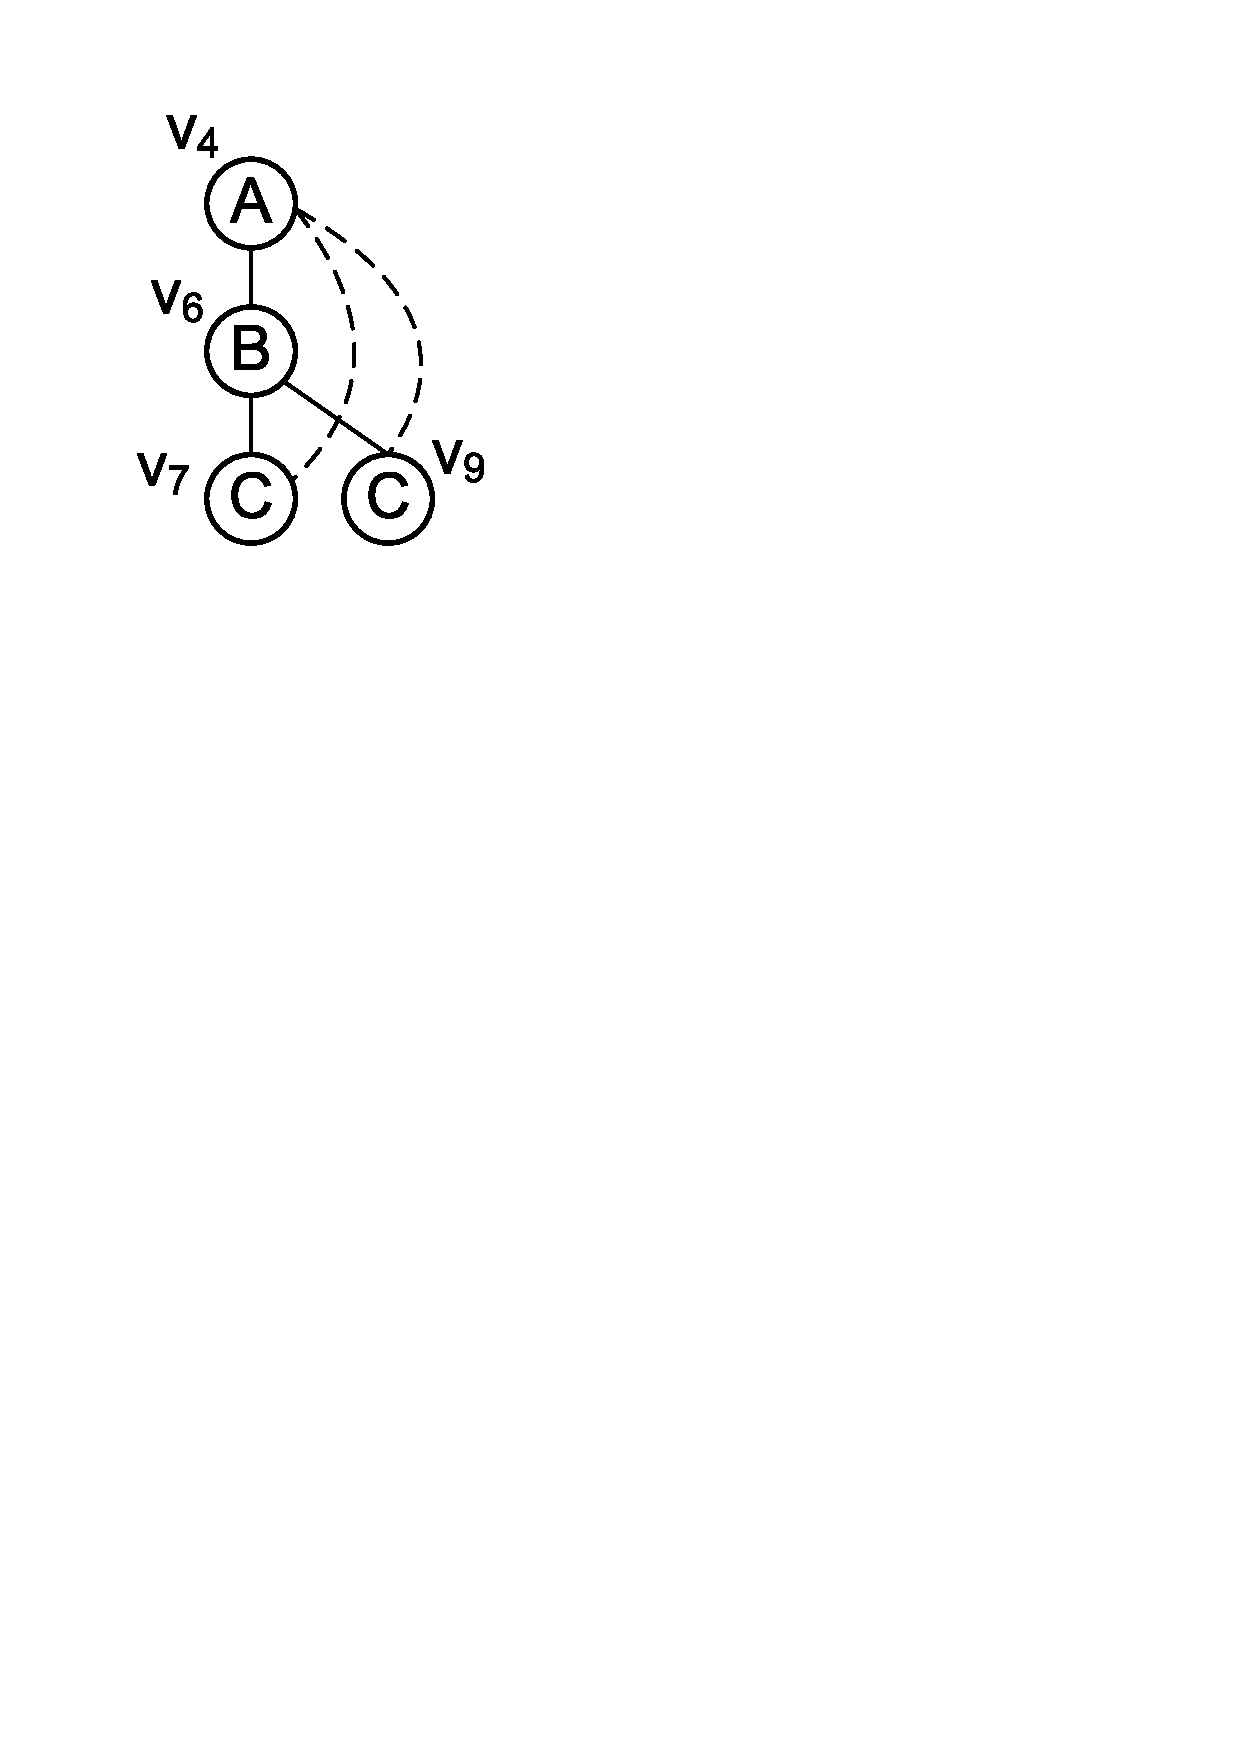
\includegraphics[scale=0.35]{images/tree_structure1}
			\label{fig:tree_structure1}
		}
		\subfigure[{\scriptsize Replica of $Q_1$}]  {
			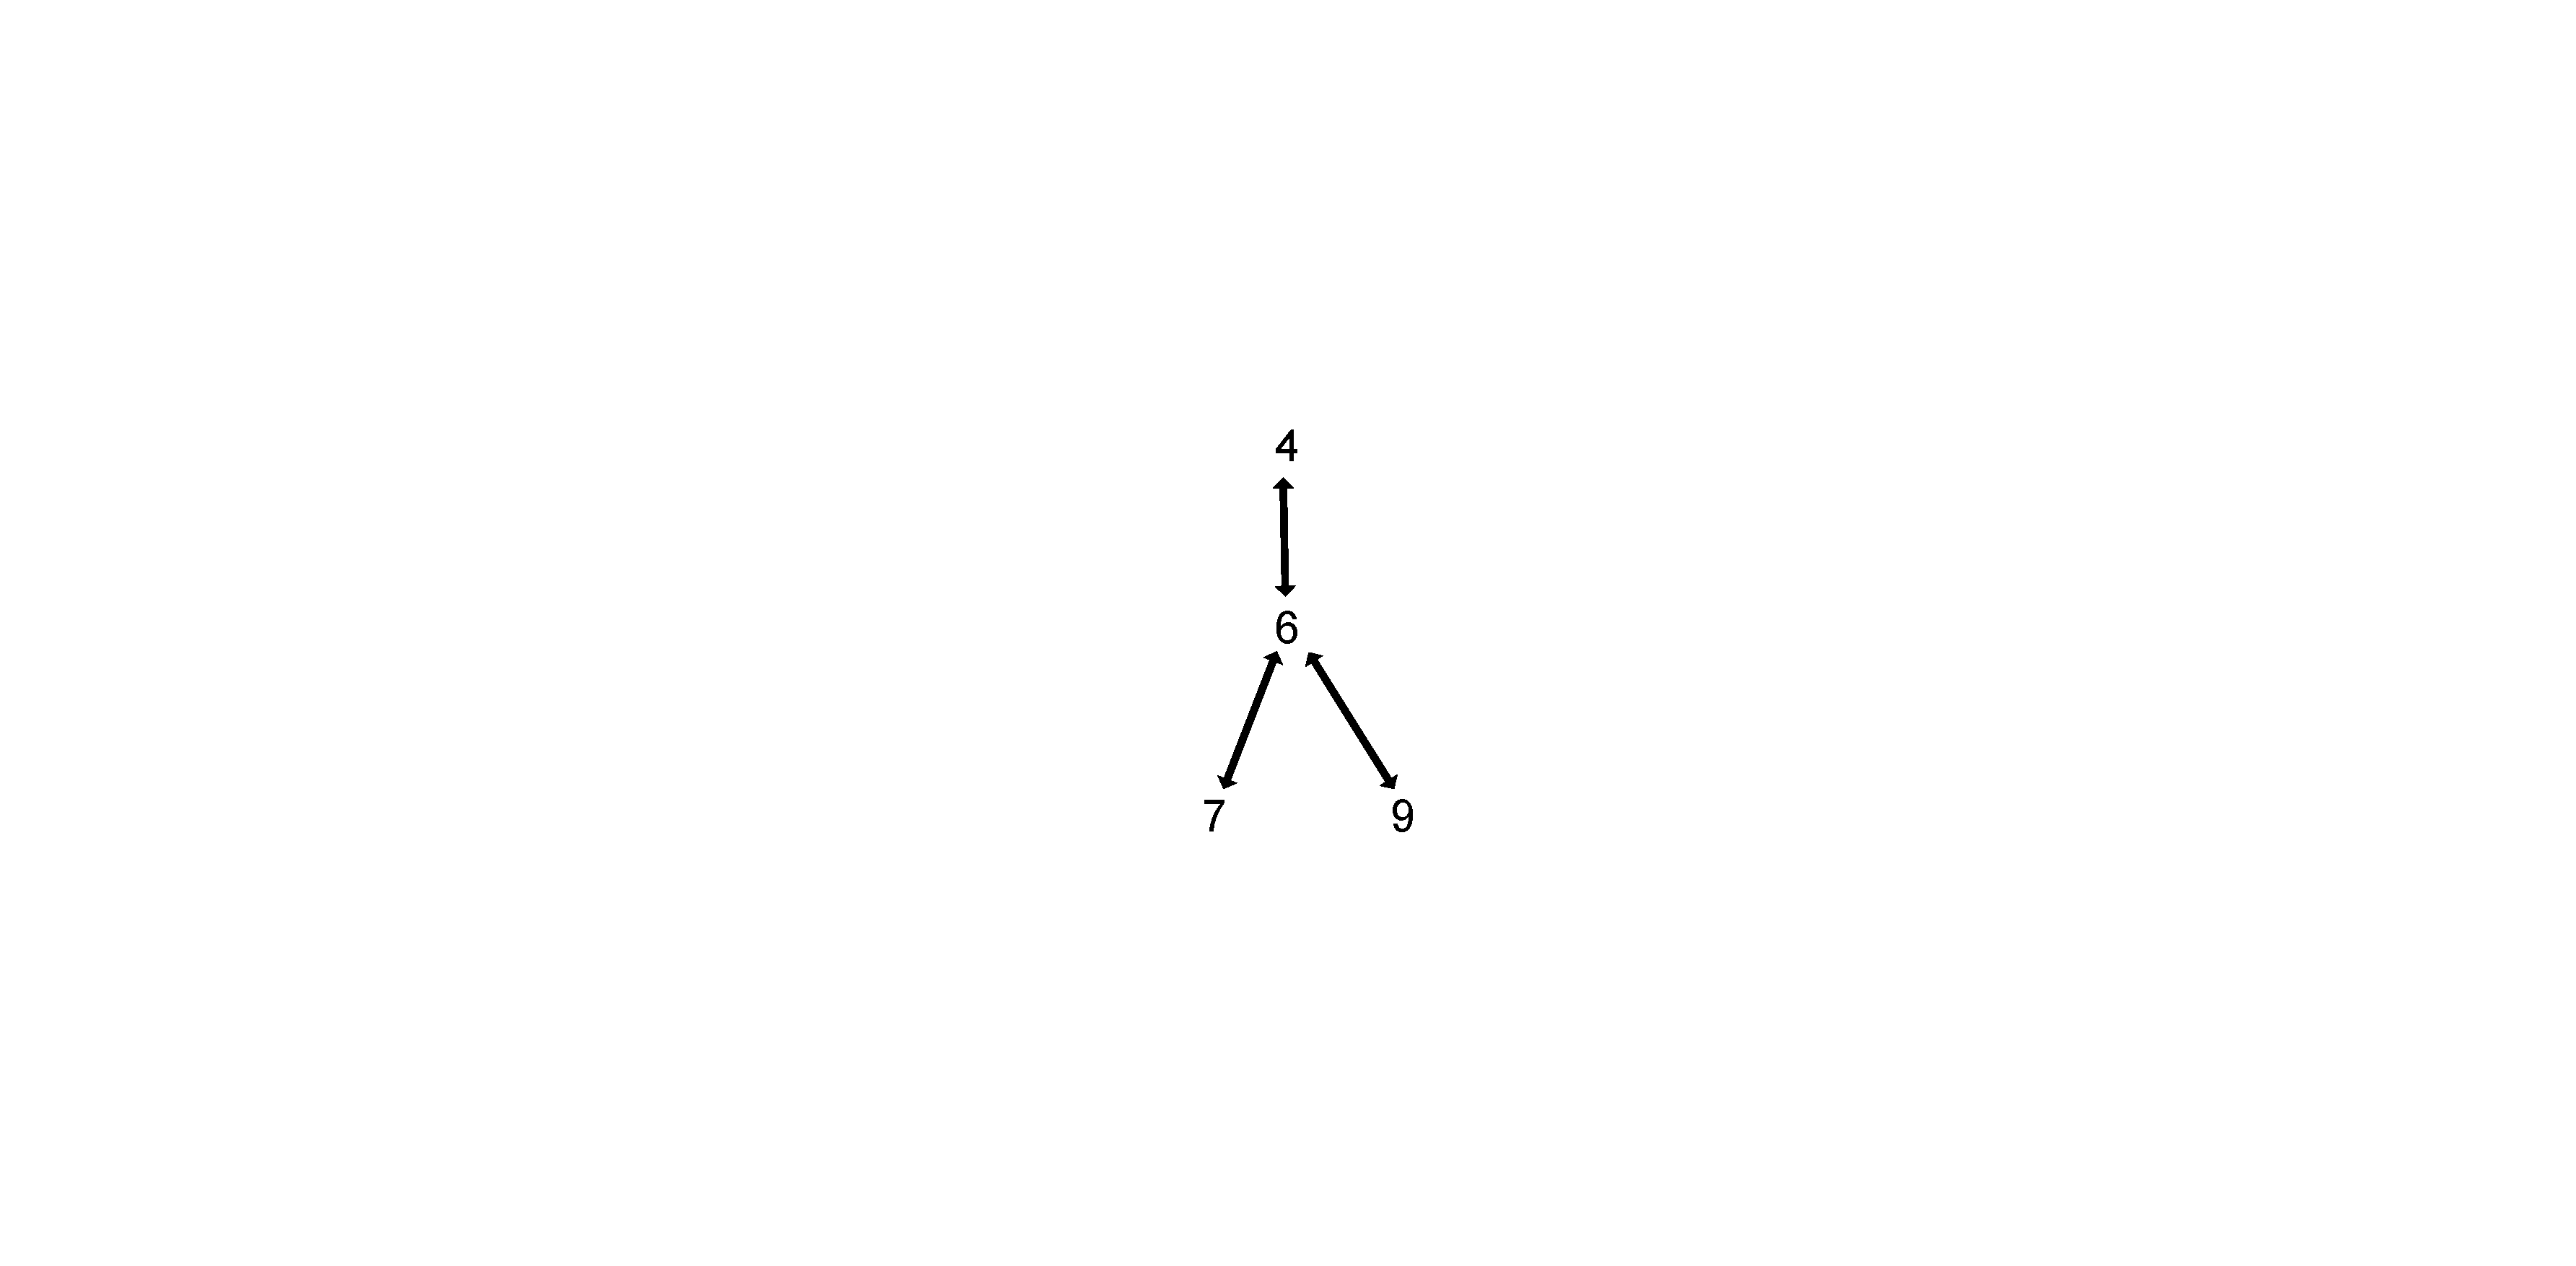
\includegraphics[scale=0.26]{images/tree_structure2}
			\label{fig:tree_structure2}
		}
	}
	\captionsetup[subfigure]{skip=5pt}
	\begin{subfigure}[b]{0.2\textwidth}
		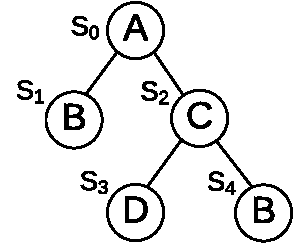
\includegraphics[scale=0.6]{img_ex/corrq2.pdf}
		\caption{}
		\label{fig:tree_structure3}
	\end{subfigure}%
	% \hspace*{\fill}
	% \subfigure[{\scriptsize Subgraph Pattern $Q_2$}]  {
	% 	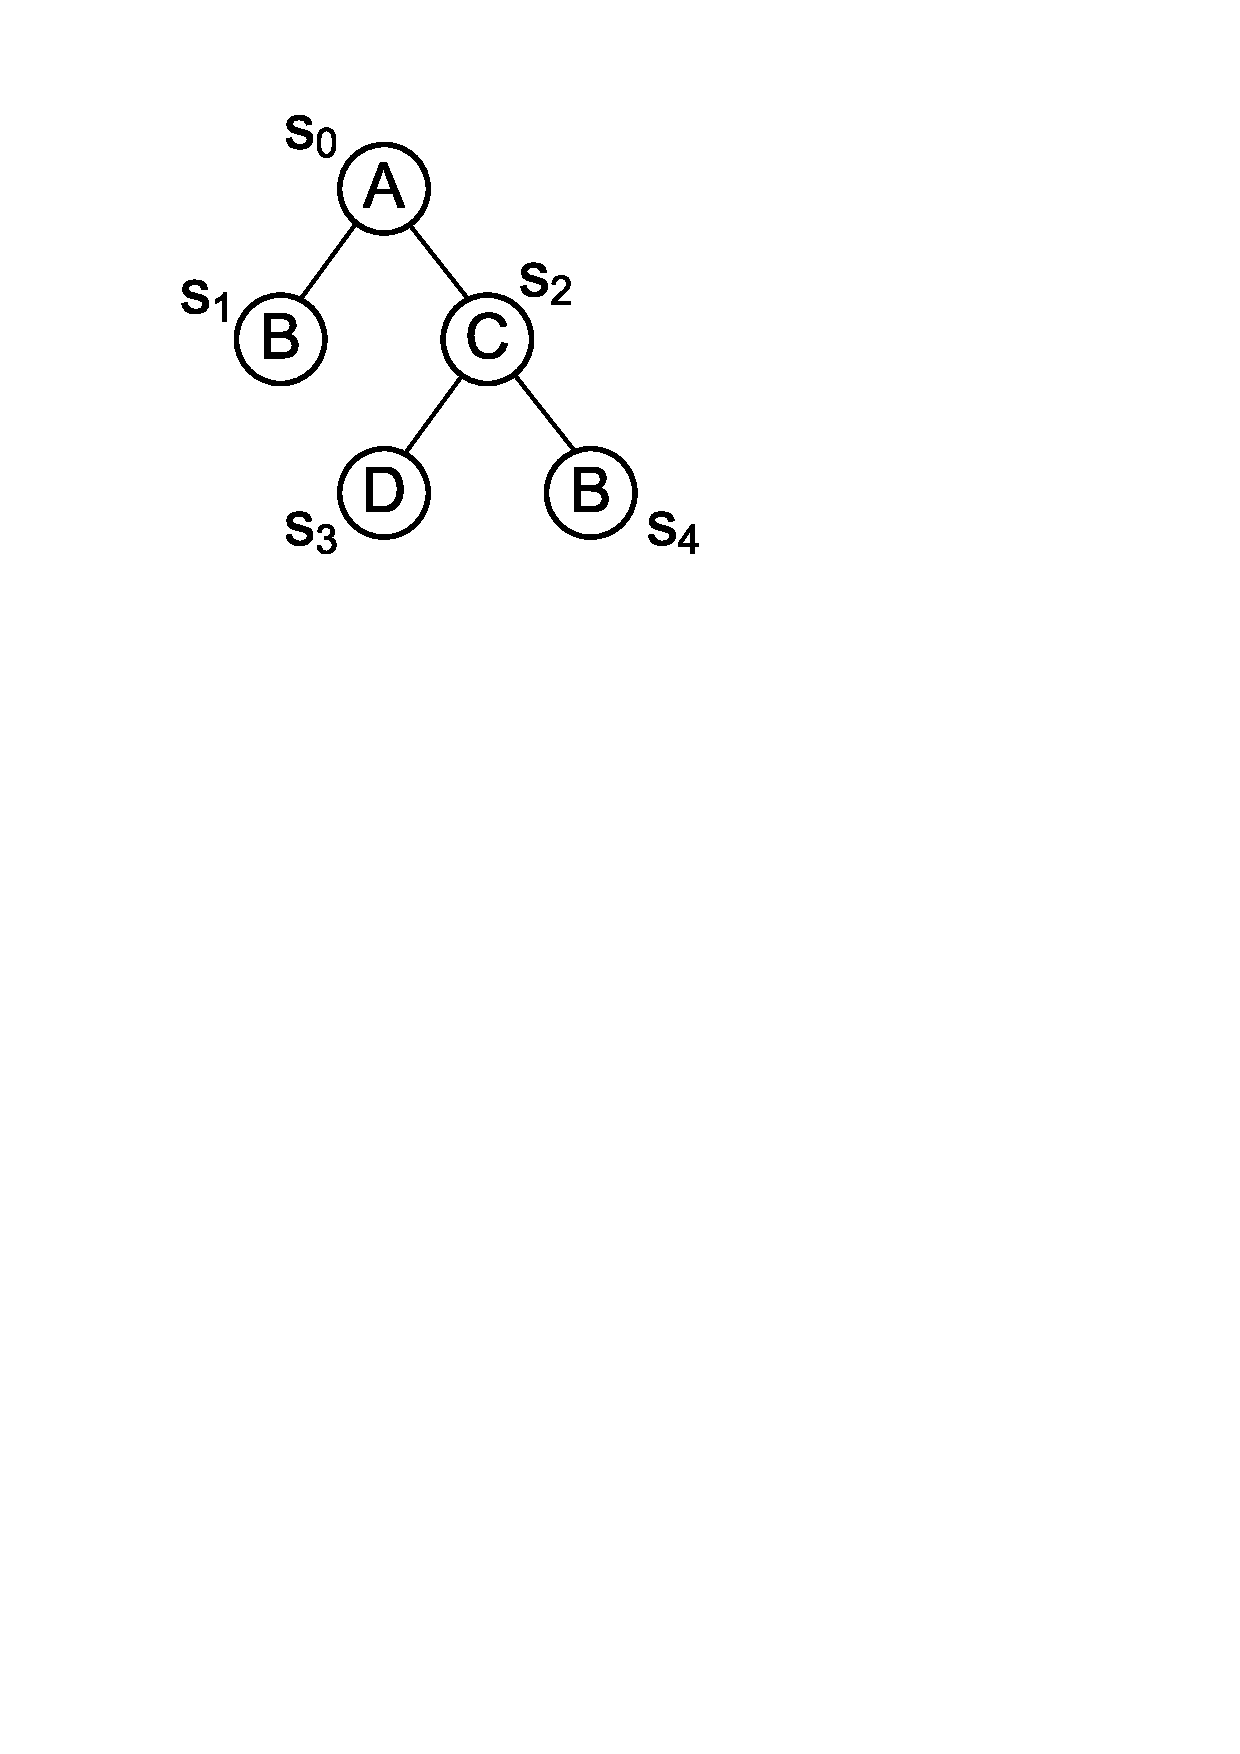
\includegraphics[scale=0.33]{images/tree_structure3}
	% 	\label{fig:tree_structure3}
	% }
	\begin{subfigure}[b]{0.25\textwidth}
		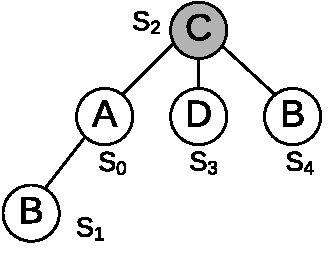
\includegraphics[scale=0.6]{img_ex/centerq2.pdf}
		\caption{}
		\label{fig:tree_structure4}
	\end{subfigure}
	% \subfigure[{\scriptsize Collection Tree of $Q_2$}] {
	% 	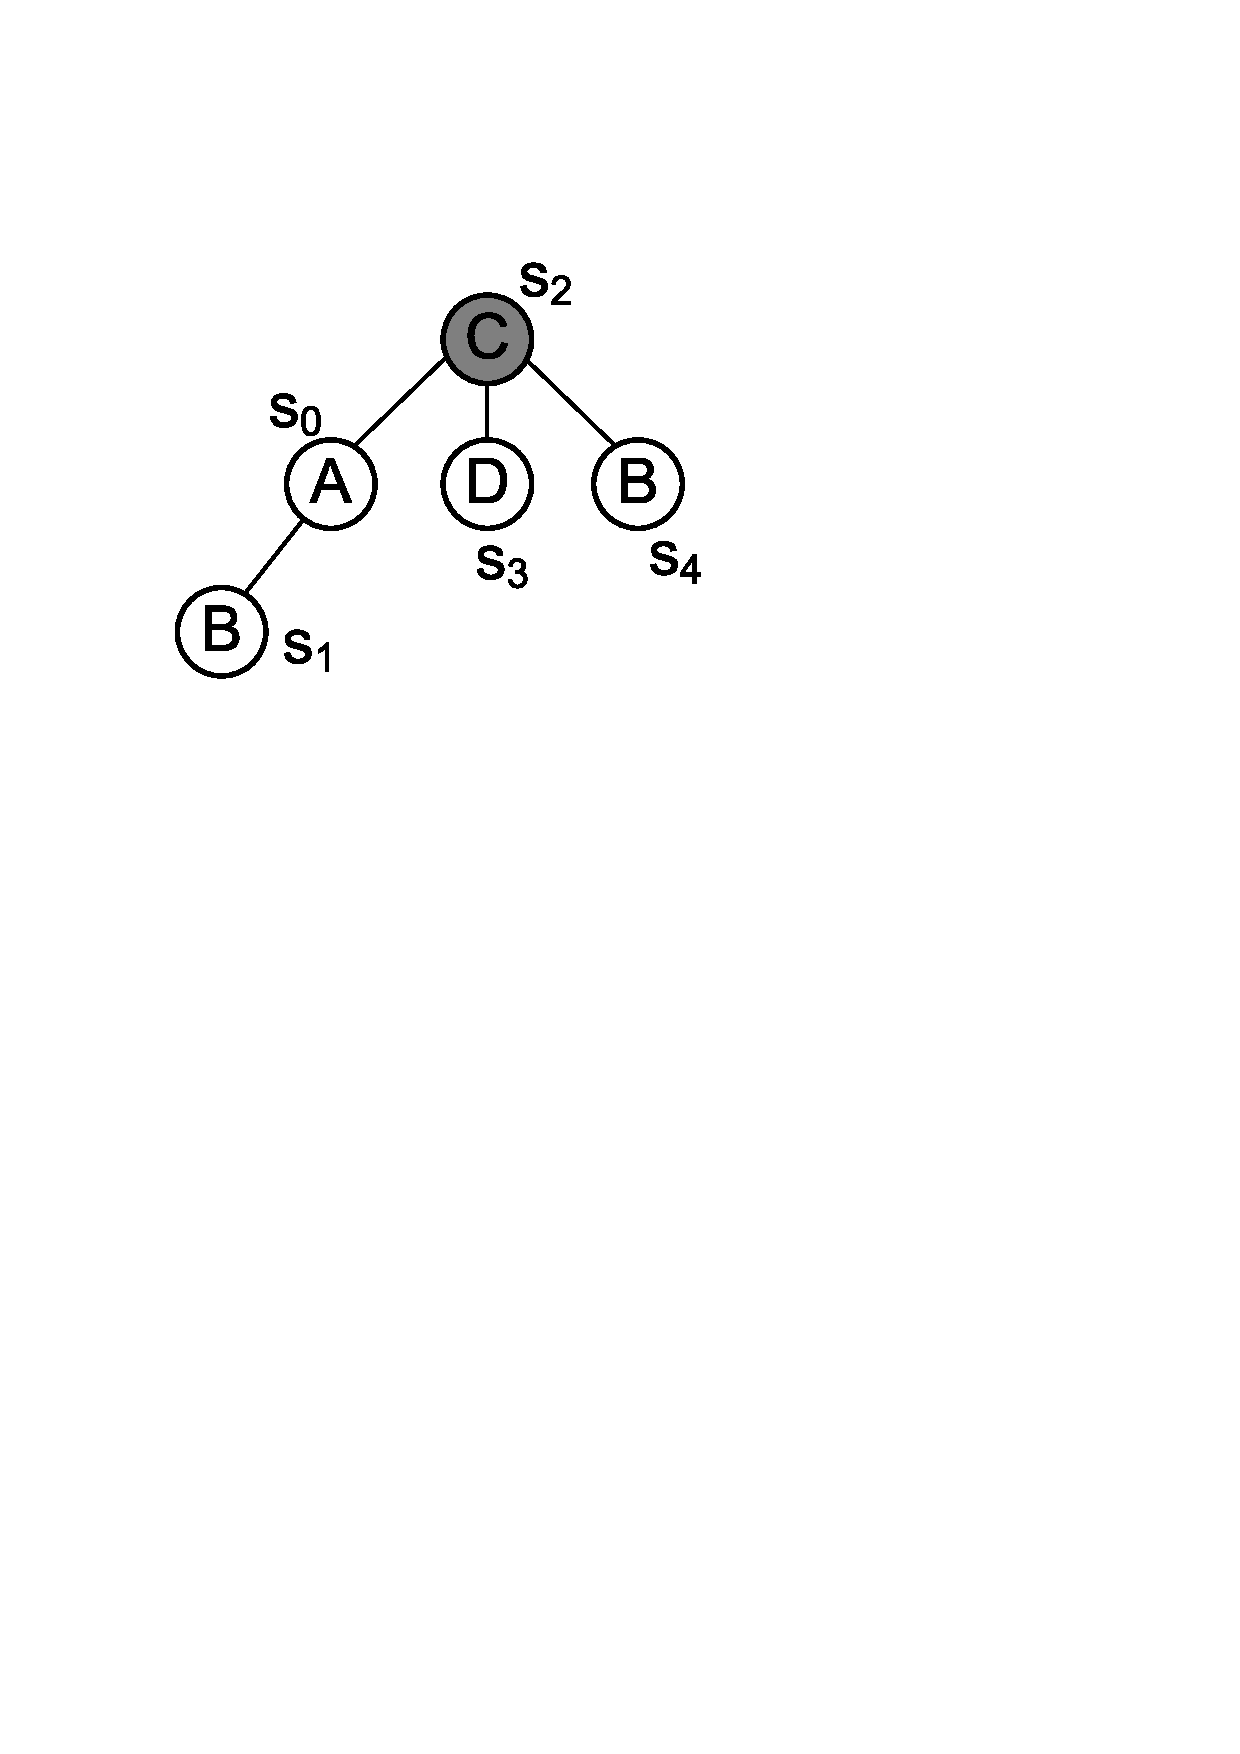
\includegraphics[scale=0.33]{images/tree_structure4}
	% 	\label{fig:tree_structure4}
	% }
	\begin{subfigure}[b]{0.5\textwidth}
		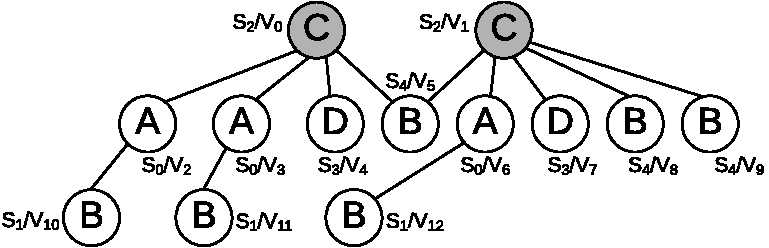
\includegraphics[scale=0.6]{img_ex/collectex.pdf}
		\caption{}
		\label{fig:tree_structure5}
	\end{subfigure}
	% \subfigure[{\scriptsize Occurrence of $Q_2$ in $G$}] {
	% 	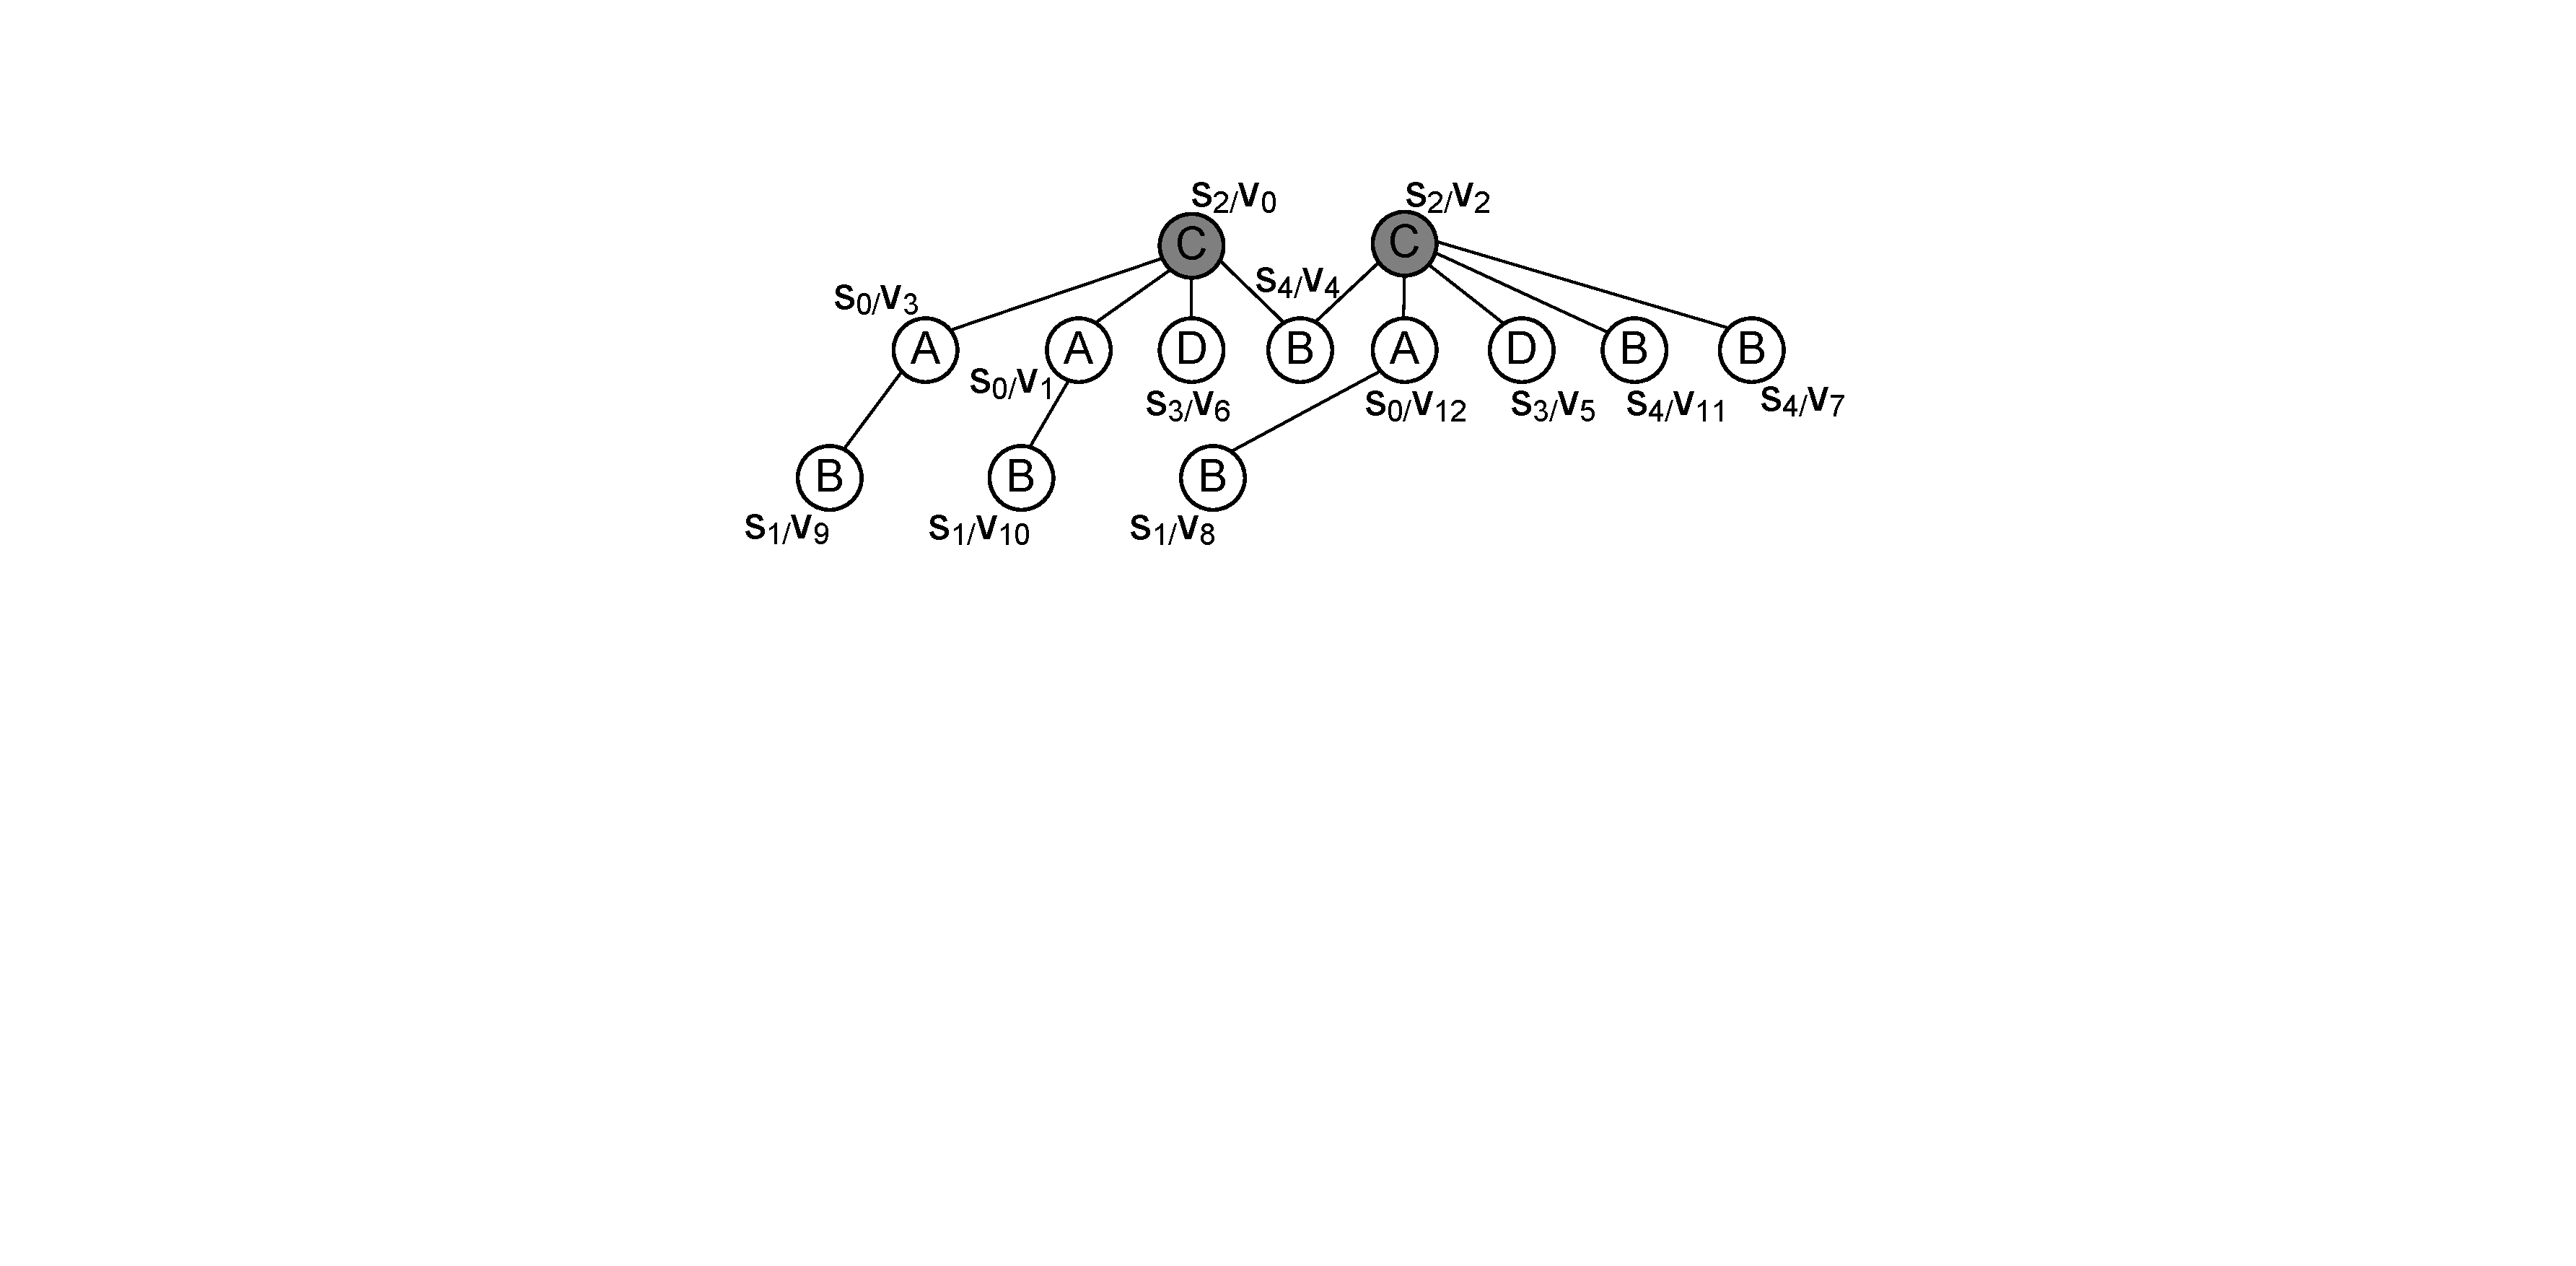
\includegraphics[scale=0.30]{images/tree_structure5}
	% 	\label{fig:tree_structure5}
	% }
	\vspace{-2mm}
	\caption{\scriptsize Figure \ref{fig:tree_structure0} is the subgraph pattern of $Q_1$, Figure \ref{fig:tree_structure2} is a replica of the occurrence of $Q_1$ in Figure \ref{fig:tree_structure1} without any backward edges (the dotted lines are the backward edges in $Q_1$). Figure \ref{fig:tree_structure4} is the same subgraph pattern $Q_2$ with Figure \ref{fig:tree_structure3}, with collection tree rooted at the group center $s_2$. Figure \ref{fig:tree_structure5} is the occurrence of $Q_2$ in data graph $G$.}
	\label{fig:replica}
	% \vspace{-5mm}
\end{figure}
% }
% ~\newline
% ~\newline

%
Then, we consider the group center as the root of the tree. During the collection, the collection is initiated from the root of the tree.

% \subsubsection{Recursive Collection}\label{subsubsec:recursive}
% The collection could be completed by a naive straight forward traversal. However, we traverse by top-bottom manner and collect by bottom-top manner. This manner could help us to reduce duplicated calculation by saving the information of all ones subtrees.

\par Prior to the correlation computations for $Q$, we first update the distance index of proximity patterns using the data of proximity vertices. That is, for all $u\in Q$, for each $v\in Cor(u)$, $CorP(v)=CorP(v)\cup Q$.
\begin{lma}
	\label{lemma:distance bidirection relation between vertices and patterns}
	Let $Q$ be a subgraph, for all $v$ in data graph $G$, if $v\in \cup CorV(u),u\in Q$, then there must exists $Q\in CorP(v)$.
\end{lma}
\par After the update of the distance index, we operate the correlation calculation of subgraph $Q$. This process includes two phases.

\spara{$\bullet$ Collection Phase:} For each group center $c\in Center(Q)$, all instances of $Q$ including $c$ are enumerated in a depth-first manner similar to the recursive instances-enumeration technique of Algorithm 2. A set union of patterns contained in $CorP(u)$ is performed across every vertex $u$ of an instance group. At the same time, every vertex $v$ in the $proximity\ vertices\ map$ of $u$ ($CorV(u)$) records the proximity of pattern $Q$ in its $proximity\ patterns\ map$ ($CorP(v)$).

\begin{align}
	Collect(c,Q)=\cup \{CorP(v)|v\in instance group\}
\end{align}
% Eventually, every group center has all the correlation corresponding to the collection tree.

\spara{$\bullet$ Counting Phase:} The correlation between patterns $Q_1$ and $Q_2$ is easily stated by calculating the count of instance groups of $Q_1$ that are positive instance group of $Q_2$.
\par Clearly, a instance group $I'_i$ of $Q_1$ is a positive instance group $Q_2$, i.e. $P(I'_i,Q_2,h)=1$ if and only if
\begin{align}
	u=groupCenter(I'_i), Q_2\in Collect(u,Q_1)
\end{align}
Then, we sum all the results to get the correlation.
\begin{align}
	\tau(Q_1,Q_2,h)=\sum_i^{\sigma(Q_1)} P(I'_i,Q_2,h)
\end{align}
Algorithm 4 summarises the steps described above.

\begin{algorithm}%[h!]
	\caption{\textsc{Operate}}\label{algo:operate}
	% \begin{algorithmic}[1]
		\dontprintsemicolon
		\nonl \textbf{Input:} Graph $G$, $Q$, $replica(Q)$, hop $h$, $CorV$, $CorP$\;
		\nonl \textbf{Output:} $\tau({Q,Q_{k},h})$, updated {\sf Top\ $k$} order\;
		% $DFS\ List\leftarrow$ get rooted {\sf DFS} of $Q$ with $center$ as $root$\;
		% \ForEach{\textup{mapping $m$ of $center$ in $replica(Q)$}}
		\ForEach{\textup{vertex $m \in Mappings(center, replica(Q))$}}
		{
			$\mathbb{I}\leftarrow$ {set of all instances $I$ such that $(center, m)\in I$}\;
			\ForEach{$u\in V(replica(Q))$ \textup{constituing an $instance$ in} $\mathbb{I}$}
			{
				$\forall v \in CorV(u)$, $CorP(v)\leftarrow CorP(v) \cup \{Q\}$\;
				$Collect(m, Q) \leftarrow Collect(m, Q) \cup CorP(u)$\;	 
			}						
		}
		\ForEach{\textup{pattern $Q_k$ in set {\sf operated}}}
		{
			% $\tau(Q, Q_k, h)\leftarrow$ number of instance group centers $m$ s.t. $Q_k\in Collect(m, Q)$\;
			$\tau(Q, Q_k, h)\leftarrow$  $|\{m$ | $m\in Mappings(center,$ $replica(Q)$) $\wedge$ $Q_k\in Collect(m, Q)\}|$\;
		}
		Update {\sf Top\ $k$} order with computed correlation ($\tau$) values\;
		{\sf operated} $\leftarrow$ {\sf operated} $\cup \ \{Q\}$\;

		% \REQUIRE data graph: $G$, hop value: $h$, initial distance index set: $Index$
		% \ENSURE
		% \STATE $DFS\ List\leftarrow$ get rooted {\sf DFS} of $Q$ with $center$ as $root$
		% \FORALL{mappings $m$ of $center$ in $replica(Q)$}
		% % \STATE $\mathbb{I}\leftarrow$ {set of all instances of $Q$ in $replica(Q)$ containing $m$ mapped to $center$}
		% \FORALL{vertex $u$ constituting an instance in $\mathbb{I}$}
		% \STATE $\forall v\in CorV(u)$, $CorP(v)\leftarrow CorP(v)\cup Q$
		% \STATE $Collect(m, Q)\leftarrow Collect(m, Q)\cup CorP(u)$
		% \ENDFOR
		% \ENDFOR
		% \FORALL{patterns $Q_k$ in set {\sf operated}}
		% \STATE $\tau(Q, Q_k, h)\leftarrow$ number of instance group centers $m$ s.t. $Q_k\in Collect(m, Q)$
		% \ENDFOR
		% \STATE Update {\sf Top\ $k$} list with the computed correlation ($\tau$) values
		% \STATE {\sf operated} $\leftarrow$ {\sf operated} $\cup \ Q$
		% \RETURN
	% \end{algorithmic}
\end{algorithm}
%append the "complete" collect-stat algorithm here 

% \begin{exple}
% 	In Figure \ref{fig:tree_structure5}, $v_0$ initiates a collection and it first goes to the deeper level until it reach the leaf, $v_9$, then it goes up from $v_9$ to $v_0$. Suppose $CorP(v_9)=\{Q_1\}$ and $CorP(v_3)=\{Q_2\}$, then $Collect(v_3,Q)=\{Q_1,Q_2\}$. This operation continues until $Collect(v_0,Q)$ is calculated. Moreover, since $Collect(v_4,Q)$ is calculated during the collection of $v_0$, it need not to be calculated again during the other collections. For example, in this case, $v_2$ initiates a collection and goes to $v_4$ and it can directly get the result of $Collect(v_4,Q)$ without going deeper.
% \end{exple}


\subsection{Avoiding Subgraph/Supergraph Correlation}\label{subsec:avoiding}
As we mentioned in Section \ref{sec:problem}, we do not want to consider the correlation of $Q_1,Q_2$ if $Q_1$ is a subgraph or a supergraph of $Q_2$. If $Q_2$ is extended from $Q_1$, we could easily know $Q_2$ is the supergraph of $Q_1$ and skip their correlation calculation. However, there are more troublesome conditions.


% \eat{
\begin{figure}[t!]
	\centering
	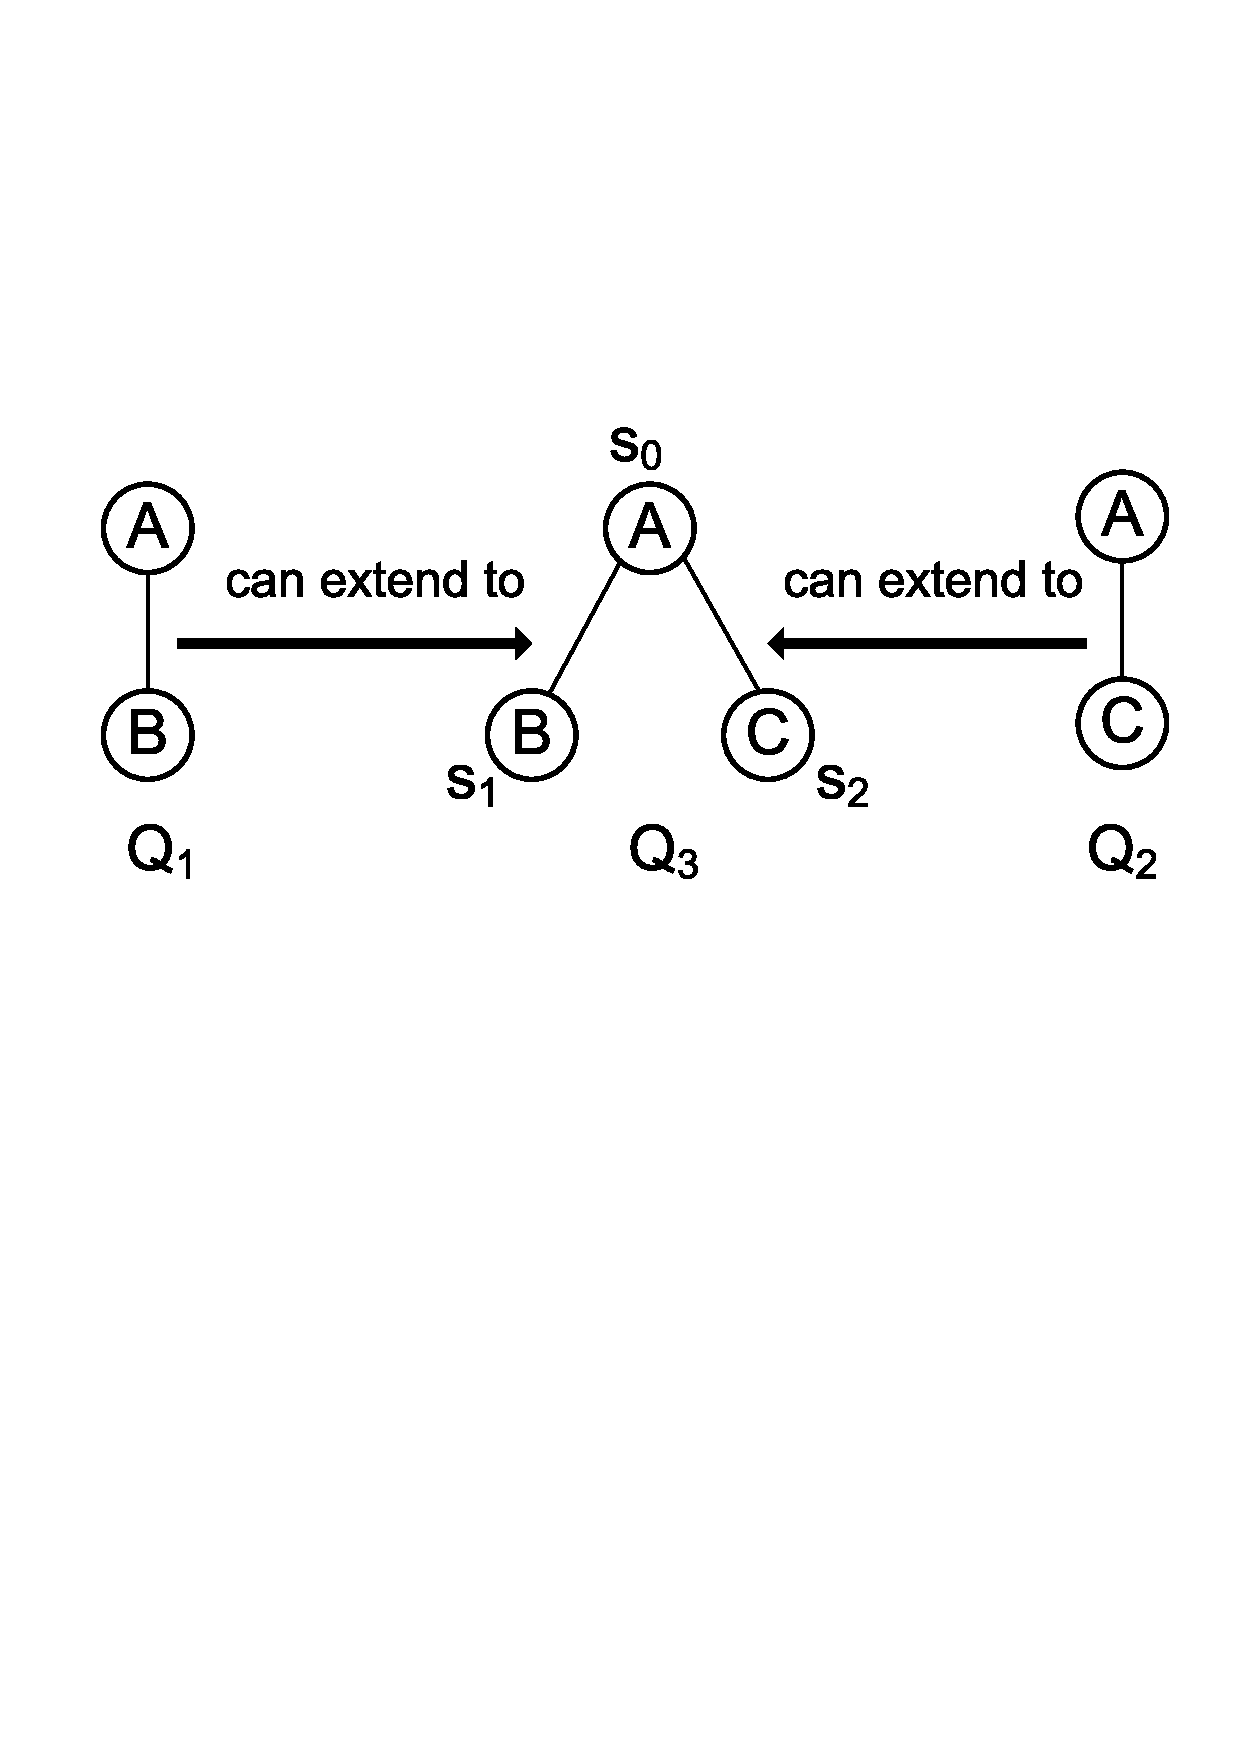
\includegraphics[scale=0.32]{images/avoiding}
	\vspace{-2mm}
	\caption{\scriptsize Subgraph $Q_1$ and $Q_2$ are the subgraphs of $Q_3$.}
	\label{fig:avoiding}
	\vspace{-4mm}
\end{figure}
% }

\begin{exple}
	In Figure \ref{fig:avoiding}, suppose $Q_1$ extended to $Q_3$ and $Q_3$ knows that $Q_1$ is its subgraph. However, during {\sf Op($Q_3$)}, $Q_3$ must avoid the correlation $\tau(Q_3,Q_2,h)$ because $Q_2$ is also the subgraph of $Q_3$.
\end{exple}


Obviously, we can not use subgraph isomorphism to check this relationship of $Q_1,Q_2$ before the correlation calculation since it is too expensive. We use following approach to rapidly get the answer.
\par We first add one more rule to best-first-search, if $\sigma(Q_1)=\sigma(Q_2)$, $Q_1$ has higher priority to be operated if and only if:
\begin{align*} |V_{Q_1}|<|V_{Q_2}| \end{align*}
According to this rule, together with downward-closure, we could always
guarantee that $Q_1$ is extended before $Q_2$. \par For each subgraph $Q$, it
maintain a subgraph set $SubRec(Q)$, recording all of its subgraphs. Under our
assumption, $Q_1$ can extend to $Q_2$ so that $Q_2$ knows that $Q_1$ is the
subgraph of $Q_2$ and all the subgraphs of $Q_1$ are also the subgraphs of
$Q_2$. As a result, if $Q_1$ can extend to $Q_2$, then we operate
$SubRec(Q_2)=SubRec(Q_2)\cap Q_1\cap SubRec(Q_1)$. As {\sf Op($Q$)} is
occurring, if $Q_i\in SubRec(Q)$, we skip $\tau(Q,Q_i,h)$.

\section{Mining Algorithm}
\label{subsec:miningalgo}
The complete mining algorithm consists of an initialization step and the search
algorithm to compute top-\textit{k} pairs of correlated subgraph patterns. The
details of these procedures are described in the following subsections.
\subsection{Initialization}
\label{subsec:initialization}
Algorithm \ref{algo:initialization} specifies the step-by-step operations of the
initialization procedure.

\begin{algorithm}%[h!]
	\caption{\textsc{Initialization}}\label{algo:initialization}
	\dontprintsemicolon
	\nonl \textbf{Input:} Graph $G$, {\sf Min-Sup:} $min\_sup$, hop value: $h$\;
	\nonl \textbf{Output:} frequent edges set: $F\_edges$, proximate vertices
	index: $CorV$, modified data graph: $G$ \;
		% $F\_edges\leftarrow$ frequent edges from $E(G)$\;
		$F\_edges\leftarrow \{e\ |\ e \in E(G),\ \sigma(e) \geq min\_sup \}$\;
		\ForEach{\textup{$u \in V(G)$ such that $(u, u')$\ \in\ F\_edges\ \ }}
		{\textsc{BFS} from $u$ to all $v\in V(G)$, such that min distance
		$d(u,v)\le h$\; $CorV(u) \leftarrow$ set of all $v$ obtained above\;}
		$NF\_edge\leftarrow E(G)\setminus F\_edge$ \; Remove $NF\_edge$ from
		$E(G)$\; \Return {$F\_edges,\ CorV,\ G$}\;
	% \end{algorithmic}
\end{algorithm}

The algorithm begins with a brute-force search to obtain all frequent edges in
the data graph (line 2). Once the set of frequent edges (stored in variable
$F\_edges$) is computed, the algorithm executes a breadth-first search (BFS)
procedure (line 4) for every vertex $u$ that constitutes an edge in $F\_edges$
to obtain all vertices satisfying the hop constraint with respect to $u$. The
set of these vertices is stored in the $CorV$ dictionary mapped to $u$ (line 5).
Thus, the set of proximate vertices for every vertex constituting a frequent
edge is obtained and stored. Finally, the algorithm deletes the set of
infrequent edges from $G$ to obtain the modified data graph (lines 7-8).
Infrequent edges are removed since these have no bearing on the algorithm
hereafter and doing so accelerates the search procedure.
% The first step is get all the frequent edges of the data graph (line ). Then,
% for every vertex of the frequent edges, we use BFS to get all the other
% vertices which satisfies the hop-constraints with it (line ). We put the
% result in the distance index set after the BFS of one vertex and we get all
% the proximity vertex set of every vertex (line ). We use this union set as the
% original distance index. This index set contains everything of proximity
% vertices but contains nothing of proximity patterns. We will use this original
% set to create and maintain the index of proximity patterns, specified in
% Section \ref{subsec:search-steps}. Finally, we remove the infrequent edges
% from the data graph (line ) because they are useless after initialization and
% removing them could accelerate the search.

\subsection{Search Steps}
\label{subsec:search-steps}
Following the initialization, the search algorithm as specified in
Algorithm~\ref{algo:searchsteps} is executed.
\begin{algorithm}
	\dontprintsemicolon
	\caption{\textsc{Search}}\label{algo:searchsteps}
	\nonl \textbf{Input:} Graph $G$, {\sf Min-Sup:} $min\_sup$, frequent edges
	set: $F\_edges$, $CorV$, Generated patterns dictionary: $\mathbb{D}$ \;
	\nonl \textbf{Output:} $top\_k$ pairs of correlated subgraph patterns  \;
	Initialize {\sf Search Queue} with $F\_edges$ \; 
	\While{\textup{\textsc{CeasingCondition} is not satisfied}} 
	{
		subgraph $Q \leftarrow$ {\sf Search\
		Queue.Pop()}\; 
		Execute \textsc{Operate($Q$)}\; 
		$Ex(Q) \leftarrow $ \textsc{SubgraphEdgeExtensions($Q$)}\; 
		\ForEach{\textup{candidate edge} $e(u,v)\in Ex(Q)$} 
		{
			child $Q'\leftarrow Q$ extended with $e$\; 
			\uIf{$DFS\ Code(Q') \notin \mathbb{D}$}
			{
				$replica(Q') \leftarrow $ \textsc{GetReplica($Q', u, e, \dots$)}\;
				Compute $\sigma(Q')$ from $replica(Q')$\;
				\uIf {$\sigma(Q')\geq min\_sup$}
				{
					Push $Q'$ into \textsc{SearchQueue}\;
				}
				Record $DFS\ Code(Q')$ in $\mathbb{D}$\;
			}
			\Else
			{
				continue\;
			}
		}
	}
		\Return {$top\_k$ \textup{correlated pairs}}\;
	% \end{algorithmic}
\end{algorithm}

The algorithm begins with the initialization of a priority queue called
$Processing\_Queue$ (line 1) that stores subgraph patterns scheduled for
correlation computation with the property that a pattern with a higher
MNI-support is accorded a higher priority following the best-first search
strategy (Section~\ref{subsubsec:estimating}). $Processing\_Queue$ is
initialized with the set of frequent edges (queued in the order of decreasing
support values). During search, as long as the $ceasing\ condition$
(Section~\ref{subsubsec:ceasing}) remains unsatisfied, the subgraph pattern at
the front of $Processing\_Queue$ is selected for correlation computation and
extension. Correlation computation takes place in method {\sf Operate}
(Algorithm~\ref{algo:operate}) wherein the top-\textit{k} set can also be
updated. This is followed by the computation of all possible one edge extensions
in $Q$ in method {\sf Subgraph Edge Extensions} (line 5). For every candidate
extension in $Ex(Q)$, the DFS Code of the resulting child subgraph pattern $Q'$
is tested for presence in dictionary $\mathbb{D}$. A match in $\mathbb{D}$
indicates that $Q'$ has already been generated previously, so the algorithm
proceeds with the MNI-support computation only if there is no match (line 8).
MNI-support computation for $Q'$ requires the construction of its $replica$
structure, which the algorithm computes and stores through the invocation of
{\sf Get Replica} method described (line 9). Note that the $replica$ structure
for a child pattern not only establishes the MNI-support but also allows
correlation computation in method {\sf Operate}. If the child pattern's
MNI-support value exceeds the threshold $min\_sup$, it is pushed into
$Processing\_Queue$ (line 12) to be (possibly) processed in a later iteration of
the outer loop. $DFS\_Code(Q')$ is recorded in $\mathbb{D}$ (line 14).
% During the search step, if the ceasing condition in Section
% \ref{subsubsec:ceasing} is not satisfied, we select a subgraph $Q$ in
% $Leaf(T)$ according to the criteria in Section \ref{subsubsec:estimating}
% (line ). Then we process event {\sf Op($Q$)}, which calculate the correlation
% of $Q$ and put the result into {\sf Top-$k$} set if it satisfies the condition
% specified in Section \ref{sec:calculation} (line ), and extend $Q$ to a larger
% subgraph with one edge growth. If the new extension $Q'$ satisfies the MNI
% support, we process event {\sf Found($Q'$)} (line ). The loop goes on until
% the ceasing condition is satisfied.\\
% \begin{observation} \label{ob:frequency} If two subgraphs have higher support
% values individually, it is very likely that the pair will also have a higher
% correlation. \end{observation}

% \begin{observation} \label{ob:dfs} For highly (e.g., top-$k$) correlated
% subgraphs mining, generally a breadth-first or a best-first exploration of the
% search space is more efficient compared to a depth-first traversal of the
% search space. \end{observation}

% Obviously, by setting $k$ to infinity can we mine all the correlated
% subgraphs. However, on the contrary, it is hard to control the value of {\sf
% Min-sup} to get the result of a particular $k$ of {\sf Top-$k$} correlated
% subgraphs. That is to say, the {\sf Min-Sup} problem can be transfered from
% {\sf Top-$k$} problem. As a result, we concentrate on {\sf Top-$k$} problem in
% the following sections. 

% \begin{figure}[t!]
% 	\vspace{2mm}
% 	\centering
% 	\subfigure[{\scriptsize Hello World }]
% 	{
% 		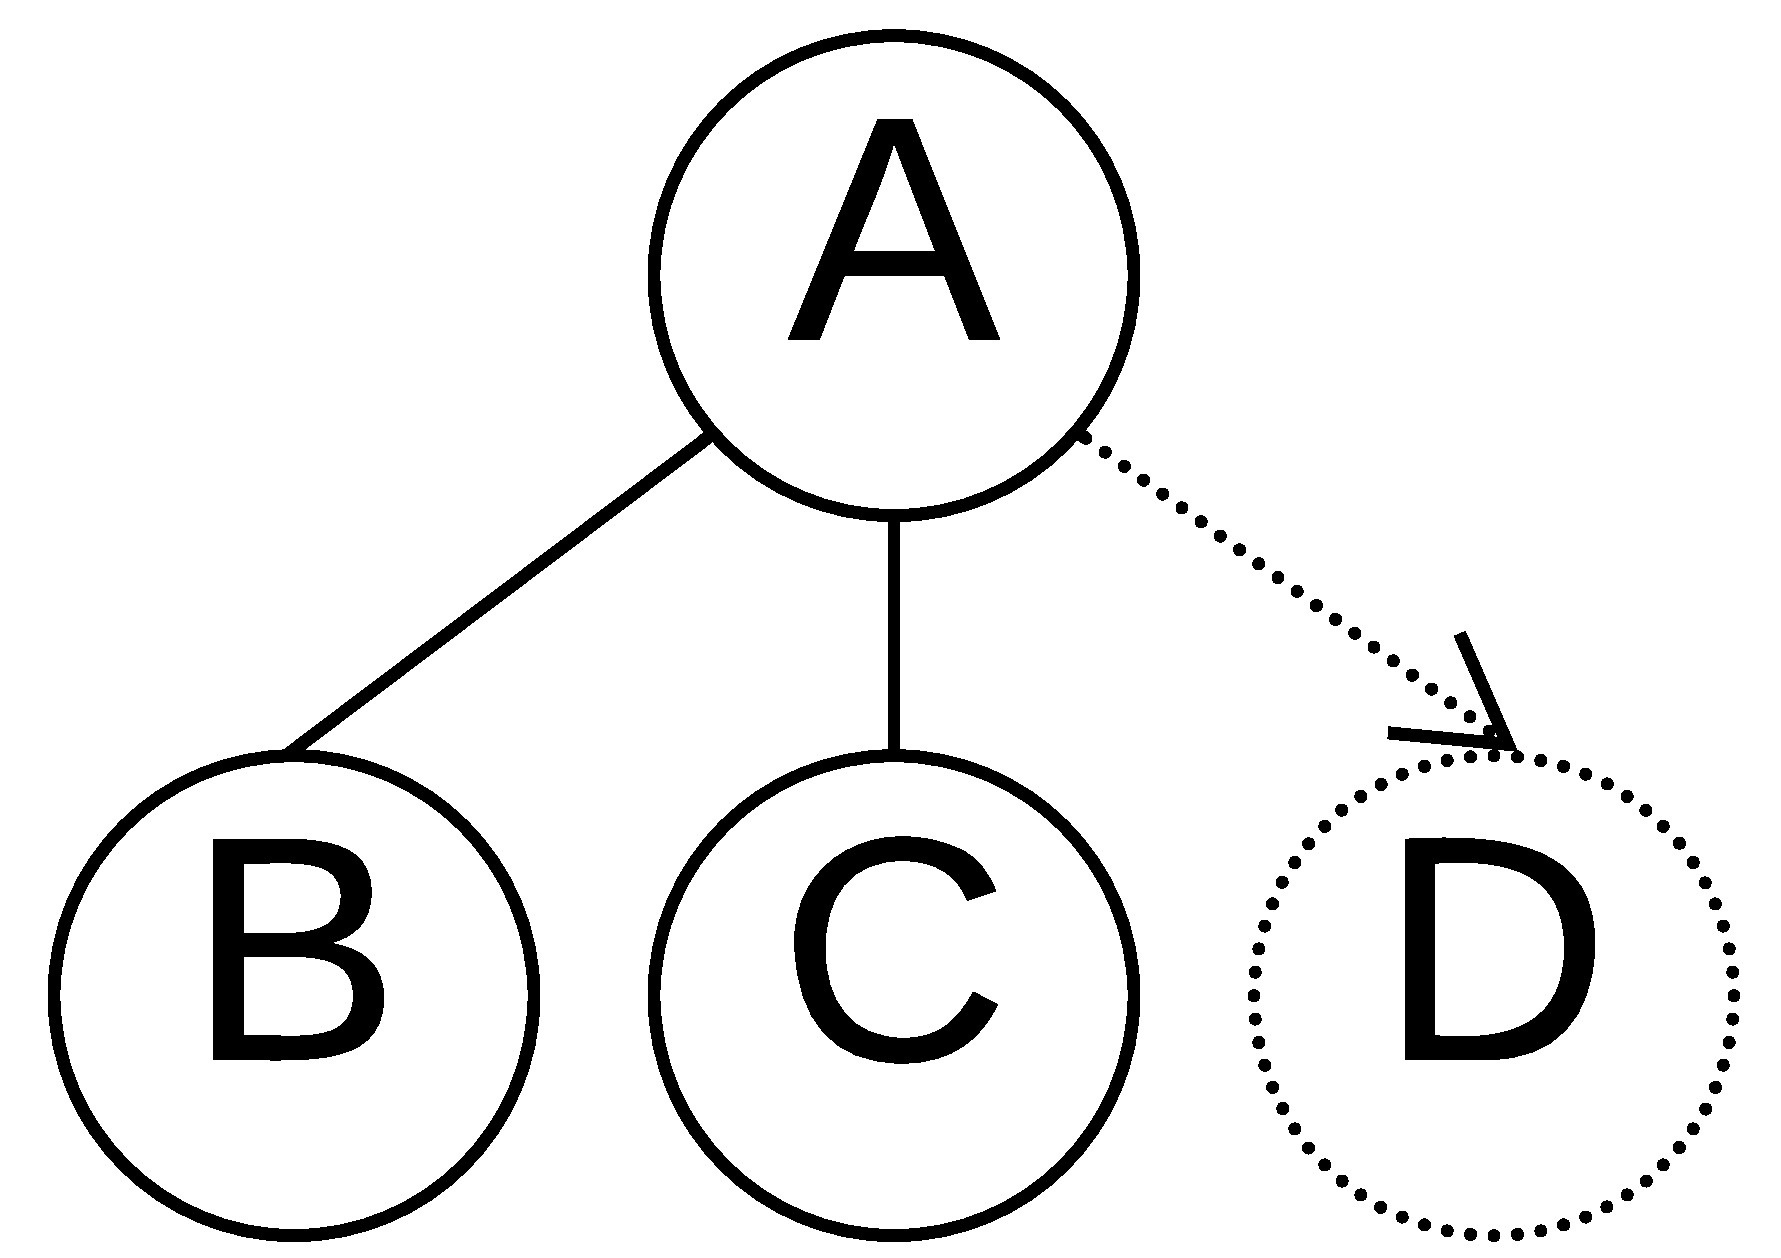
\includegraphics[scale=0.06]{img_ex/temp1.pdf}
% 		\label{subfig:exp_temp1}
% 	}
% 	\vspace{-2mm}
% 	\caption{\scriptsize Get Replica}
% 	\label{fig:exp_temp1}
% 	\vspace{-2mm}
% \end{figure}

\eat{
\begin{figure}[t!]
	\centering
	% \addtolength{\subfigbottomskip}{-5pt}
	\subfigure[{\scriptsize Subfig1}]	
	{
		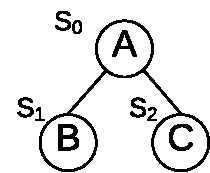
\includegraphics[scale=0.6]{img_ex/Exact-Q.pdf}
		\label {subfig:exact_Q}
	}
	% \newcommand{\subfigbottomskip}{100pt}
	\subfigure[{\scriptsize Subfig2}]
	{
		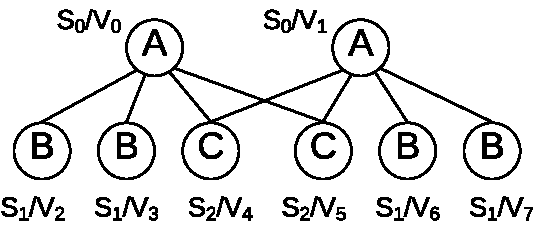
\includegraphics[scale=0.6]{img_ex/Exact-rep(Q).pdf}
		\label {subfig:exact_repQ}
	}
	\vspace{-2mm}
	\caption{\scriptsize GetReplica}
	\label{fig:avoiding}
	\vspace{-6mm}
\end{figure}
}

% \begin{figure}
% 	\begin{subfigure}[b]{0.10\textwidth}
% 			\includegraphics[scale=0.2]{example-image-a}
% 			\caption{A gull}
% 			\label{fig:gull}
% 	\end{subfigure}%
% 	\begin{subfigure}[b]{0.10\textwidth}
% 			\includegraphics[scale=0.2]{example-image-a}
% 			\caption{A gull2}
% 			\label{fig:gull2}
% 	\end{subfigure}%
% 	\begin{subfigure}[b]{0.10\textwidth}
% 			\includegraphics[scale=0.2]{example-image-a}
% 			\caption{A tiger}
% 			\label{fig:tiger}
% 	\end{subfigure}%
% 	\begin{subfigure}[b]{0.10\textwidth}
% 			\includegraphics[scale=0.2]{example-image-a}
% 			\caption{A mouse}
% 			\label{fig:mouse}
% 	\end{subfigure}
% 	\caption{Pictures of animals}\label{fig:animals}
% \end{figure}

